%definira klasu dokumenta 
\documentclass[12pt]{report} 

%prostor izmedu naredbi \documentclass i \begin{document} se zove uvod. U njemu se nalaze naredbe koje se odnose na cijeli dokument

%osnovni LaTex ne može riješiti sve probleme, pa se koriste različiti paketi koji olakšavaju izradu željenog dokumenta
\usepackage[croatian]{babel} 
\usepackage{amssymb}
\usepackage{amsmath}
\usepackage{txfonts}
\usepackage{mathdots}
\usepackage{titlesec}
\usepackage{array}
\usepackage{lastpage}
\usepackage{etoolbox}
\usepackage{longtable, tabu}
\usepackage{color, colortbl}
\usepackage{adjustbox}
\usepackage{geometry}
\usepackage[classicReIm]{kpfonts}
\usepackage{hyperref}
\usepackage{fancyhdr}

\usepackage{float}
\usepackage{setspace}
\restylefloat{table}


\patchcmd{\chapter}{\thispagestyle{plain}}{\thispagestyle{fancy}}{}{} %redefiniranje stila stranice u paketu fancyhdr

%oblik naslova poglavlja
\titleformat{\chapter}{\normalfont\huge\bfseries}{\thechapter.}{20pt}{\Huge}
\titlespacing{\chapter}{0pt}{0pt}{40pt}


\linespread{1.3} %razmak između redaka

\geometry{a4paper, left=1in, top=1in,}  %oblik stranice

\hypersetup{ colorlinks, citecolor=black, filecolor=black, linkcolor=black,	urlcolor=black }   %izgled poveznice


%prored smanjen između redaka u nabrajanjima i popisima
\newenvironment{packed_enum}{
	\begin{enumerate}
		\setlength{\itemsep}{0pt}
		\setlength{\parskip}{0pt}
		\setlength{\parsep}{0pt}
	}{\end{enumerate}}

\newenvironment{packed_item}{
	\begin{itemize}
		\setlength{\itemsep}{0pt}
		\setlength{\parskip}{0pt}
		\setlength{\parsep}{0pt}
	}{\end{itemize}}


%boja za privatni i udaljeni kljuc u tablicama
\definecolor{LightBlue}{rgb}{0.9,0.9,1}
\definecolor{LightGreen}{rgb}{0.9,1,0.9}


%podesavanje zaglavlja i podnožja

\pagestyle{fancy}
\lhead{Programsko inženjerstvo}
\rhead{$<$Projektni zadatak$>$}
\lfoot{$<$Naziv grupe$>$}
\cfoot{stranica \thepage/\pageref{LastPage}}
\rfoot{\today}
\renewcommand{\headrulewidth}{0.2pt}
\renewcommand{\footrulewidth}{0.2pt}


\begin{document} 
	
	
	
	\begin{titlepage}
		\begin{center}
			\vspace*{\stretch{1.0}} %u kombinaciji s ostalim \vspace naredbama definira razmak između redaka teksta
			\LARGE Programsko inženjerstvo\\
			\large Ak. god. 2020./2021.\\
			
			\vspace*{\stretch{3.0}}
			
			\huge $<$Naziv projekta$>$\\
			\Large Dokumentacija, Rev. \textit{$<$1 ili 2$>$}\\
			
			\vspace*{\stretch{12.0}}
			\normalsize
			Grupa: \textit{$<$Naziv grupe$>$}\\
			Voditelj: \textit{$<$Ime i prezime voditelja$>$}\\
			
			
			\vspace*{\stretch{1.0}}
			Datum predaje: \textit{$<$dan$>$. $<$mjesec$>$. $<$godina$>$.}\\
	
			\vspace*{\stretch{4.0}}
			
			Nastavnik: \textit{$<$Ime i prezime nastavnika zaduženog za vašu grupu$>$}\\
		
		\end{center}

	
	\end{titlepage}

	
	\tableofcontents

	\chapter{Dnevnik promjena dokumentacije}
		
		\textbf{\textit{Kontinuirano osvježavanje}}\\
				
		
		\begin{longtabu} to \textwidth {|X[2, l]|X[13, l]|X[3, l]|X[3, l]|}
			\hline \multicolumn{1}{|l|}{\textbf{Rev.}}	& \multicolumn{1}{l|}{\textbf{Opis promjene/dodatka}} & \multicolumn{1}{|l|}{\textbf{Autori}} & \multicolumn{1}{l|}{\textbf{Datum}} \\[3pt] \hline
			\endfirsthead
			
			\hline \multicolumn{1}{|l|}{\textbf{Rev.}}	& \multicolumn{1}{l|}{\textbf{Opis promjene/dodatka}} & \multicolumn{1}{|l|}{\textbf{Autori}} & \multicolumn{1}{l|}{\textbf{Datum}} \\[3pt] \hline
			\endhead
			
			\hline 
			\endlastfoot
			
			0.1 & Dopunjen predložak	& Rabuzin & 11.10.2020. 		\\[3pt]
			\hline
			0.2 & Opis projektnog zadatka	& Rabuzin i Šarić & 15.10.2020. 		\\[3pt]
			\hline 
			0.2.1 & Detaljnije razrađen opis projektnog zadatka	& Rabuzin i Šarić & 17.10.2020. 		\\[3pt]
			\hline 
			%U komentarima je ostavljeno kako je izgledao predložak radi reference za budućnost
			%0.2	& Dopisane upute za povijest dokumentacije.\newline Dodane reference. & Jović & 24.08.2013. 	\\[3pt] \hline 
			%0.5 & Dodan \textit{Use Case} dijagram i jedan sekvencijski dijagram, funkcionalni i nefunkcionalni zahtjevi i dodatak A & Ivošević & 25.08.2013. \\[3pt] \hline 
			%0.6 & Arhitektura i dizajn sustava, algoritmi i strukture podataka & Grudenić & 26.08.2013. \\[3pt] \hline 
			%0.8 & Povijest rada i trenutni status implementacije,\newline Zaključci i plan daljnjeg rada & Ivošević & 28.08.2013. \\[3pt] \hline 
			%0.9 & Opisi obrazaca uporabe & Jović & 07.09.2013. \\[3pt] \hline 
			%0.10 & Preveden uvod & Jović & 08.09.2013. \\[3pt] \hline 
			%0.11 & Sekvencijski dijagrami & Žužak & 09.09.2013. \\[3pt] \hline 
			%0.12.1 & Započeo dijagrame razreda & Horvat & 10.09.2013. \\[3pt] \hline 
			%0.12.2 & Nastavak dijagrama razreda & Horvat & 11.09.2013. \\[3pt] \hline 
			%\textbf{1.0} & Verzija samo s bitnim dijelovima za 1. ciklus & Ivošević & 11.09.2013. \\[3pt] \hline 
			%1.1 & Uređivanje teksta -- funkcionalni i nefunkcionalni zahtjevi & Grudenić \newline Jović & 14.09.2013. \\[3pt] \hline 
			%1.2 & Manje izmjene:Timer - Brojilo vremena & Grudenić & 15.09.2013. \\[3pt] \hline 
			%1.3 & Popravljeni dijagrami obrazaca uporabe & Jović & 15.09.2013. \\[3pt] \hline 
			%1.5 & Generalna revizija strukture dokumenta & Ivošević & 19.09.2013. \\[3pt] \hline 
			%1.5.1 & Manja revizija (dijagram razmještaja) & Jović & 20.09.2013. \\[3pt] \hline 
			%\textbf{2.0} & Konačni tekst predloška dokumentacije  & Ivošević & 28.09.2013. \\[3pt] \hline 
			&  &  & \\[3pt] \hline
			
			
		\end{longtabu}
	
	
		\textit{Moraju postojati glavne revizije dokumenata 1.0 i 2.0 na kraju prvog i drugog ciklusa. Između tih revizija mogu postojati manje revizije već prema tome kako se dokument bude nadopunjavao. Očekuje se da nakon svake značajnije promjene (dodatka, izmjene, uklanjanja dijelova teksta i popratnih grafičkih sadržaja) dokumenta se to zabilježi kao revizija. Npr., revizije unutar prvog ciklusa će imati oznake 0.1, 0.2, …, 0.9, 0.10, 0.11.. sve do konačne revizije prvog ciklusa 1.0. U drugom ciklusu se nastavlja s revizijama 1.1, 1.2, itd.}
	\chapter{Opis projektnog zadatka}
		
		\textbf{\textit{dio 1. revizije}}\\
		
		\textit{Na osnovi projektnog zadatka detaljno opisati korisničke zahtjeve. Što jasnije opisati cilj projektnog zadatka, razraditi problematiku zadatka, dodati nove aspekte problema i potencijalnih rješenja. Očekuje se minimalno 3, a poželjno 4-5 stranica opisa.	Teme koje treba dodatno razraditi u ovom poglavlju su:}
		\begin{packed_item}
			\item \textit{potencijalna korist ovog projekta}
			\item \textit{postojeća slična rješenja (istražiti i ukratko opisati razlike u odnosu na zadani zadatak). Dodajte slike koja predočavaju slična rješenja.}
			\item \textit{skup korisnika koji bi mogao biti zainteresiran za ostvareno rješenje.}
			\item \textit{mogućnost prilagodbe rješenja }
			\item \textit{opseg projektnog zadatka}
			\item \textit{moguće nadogradnje projektnog zadatka}
		\end{packed_item}
		
		\textit{Za pomoć pogledati reference navedene u poglavlju „Popis literature“, a po potrebi konzultirati sadržaj na internetu koji nudi dobre smjernice u tom pogledu.}
		\eject
		
		\section{Primjeri u \LaTeX u}
		
		\textit{Ovo potpoglavlje izbrisati.}\\

		U nastavku se nalaze različiti primjeri kako koristiti osnovne funkcionalnosti \LaTeX a koje su potrebne za izradu dokumentacije. Za dodatnu pomoć obratiti se asistentu na projektu ili potražiti upute na sljedećim web sjedištima:
		\begin{itemize}
			\item Upute za izradu diplomskog rada u \LaTeX u - \url{https://www.fer.unizg.hr/_download/repository/LaTeX-upute.pdf}
			\item \LaTeX\ projekt - \url{https://www.latex-project.org/help/}
			\item StackExchange za Tex - \url{https://tex.stackexchange.com/}\\
		
		\end{itemize} 	


		
		\noindent \underbar{podcrtani tekst}, \textbf{podebljani tekst}, 	\textit{nagnuti tekst}\\
		\noindent \normalsize primjer \large primjer \Large primjer \LARGE {primjer} \huge {primjer} \Huge primjer \normalsize
				
		\begin{packed_item}
			
			\item  primjer
			\item  primjer
			\item  primjer
			\item[] \begin{packed_enum}
				\item primjer
				\item[] \begin{packed_enum}
					\item[1.a] primjer
					\item[b] primjer
				\end{packed_enum}
				\item primjer
			\end{packed_enum}
			
		\end{packed_item}
		
		\noindent primjer url-a: \url{https://www.fer.unizg.hr/predmet/proinz/projekt}
		
		\noindent posebni znakovi: \# \$ \% \& \{ \} \_ 
		$|$ $<$ $>$ 
		\^{} 
		\~{} 
		$\backslash$ 
		
		\begin{longtabu} to \textwidth {|X[8, l]|X[8, l]|X[16, l]|} %definicija širine tablice, širine stupaca i poravnanje
			
			%definicija naslova tablice
			\hline \multicolumn{3}{|c|}{\textbf{naslov unutar tablice}}	 \\[3pt] \hline
			\endfirsthead
			
			%definicija naslova tablice prilikom prijeloma
			\hline \multicolumn{3}{|c|}{\textbf{naslov unutar tablice}}	 \\[3pt] \hline
			\endhead
			
			\hline 
			\endlastfoot
			
			\rowcolor{LightGreen}IDKorisnik & INT	&  	Lorem ipsum dolor sit amet, consectetur adipiscing elit, sed do eiusmod  	\\ \hline
			korisnickoIme	& VARCHAR &   	\\ \hline 
			email & VARCHAR &   \\ \hline 
			ime & VARCHAR	&  		\\ \hline 
			\cellcolor{LightBlue} primjer	& VARCHAR &   	\\ \hline 
			
		\end{longtabu}
		

		\begin{table}[H]
			
			\begin{longtabu} to \textwidth {|X[8, l]|X[8, l]|X[16, l]|} 
				
				\hline 
				\endfirsthead
				
				\hline 
				\endhead
				
				\hline 
				\endlastfoot
				
				\rowcolor{LightGreen}IDKorisnik & INT	&  	Lorem ipsum dolor sit amet, consectetur adipiscing elit, sed do eiusmod  	\\ \hline
				korisnickoIme	& VARCHAR &   	\\ \hline 
				email & VARCHAR &   \\ \hline 
				ime & VARCHAR	&  		\\ \hline 
				\cellcolor{LightBlue} primjer	& VARCHAR &   	\\ \hline 
				
				
			\end{longtabu}
	
			\caption{\label{tab:referencatablica} Naslov ispod tablice.}
		\end{table}
		
		
		%unos slike
		\begin{figure}[H]
			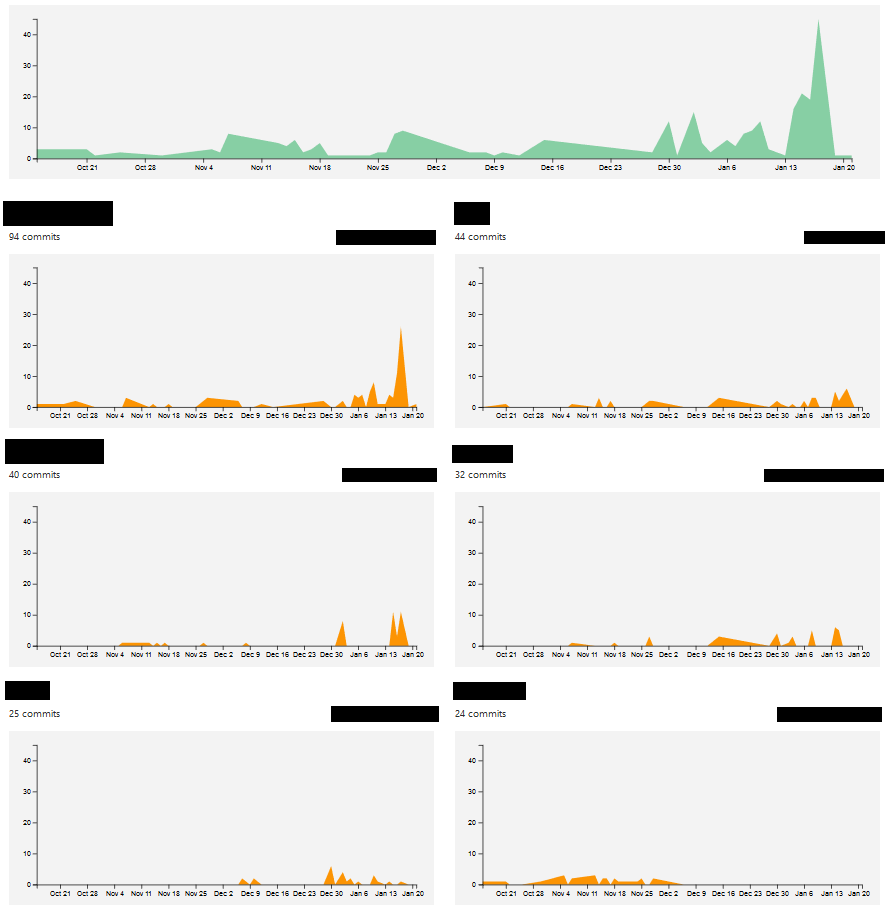
\includegraphics[scale=0.4]{slike/aktivnost.PNG} %veličina slike u odnosu na originalnu datoteku i pozicija slike
			\centering
			\caption{Primjer slike s potpisom}
			\label{fig:promjene}
		\end{figure}
		
		\begin{figure}[H]
			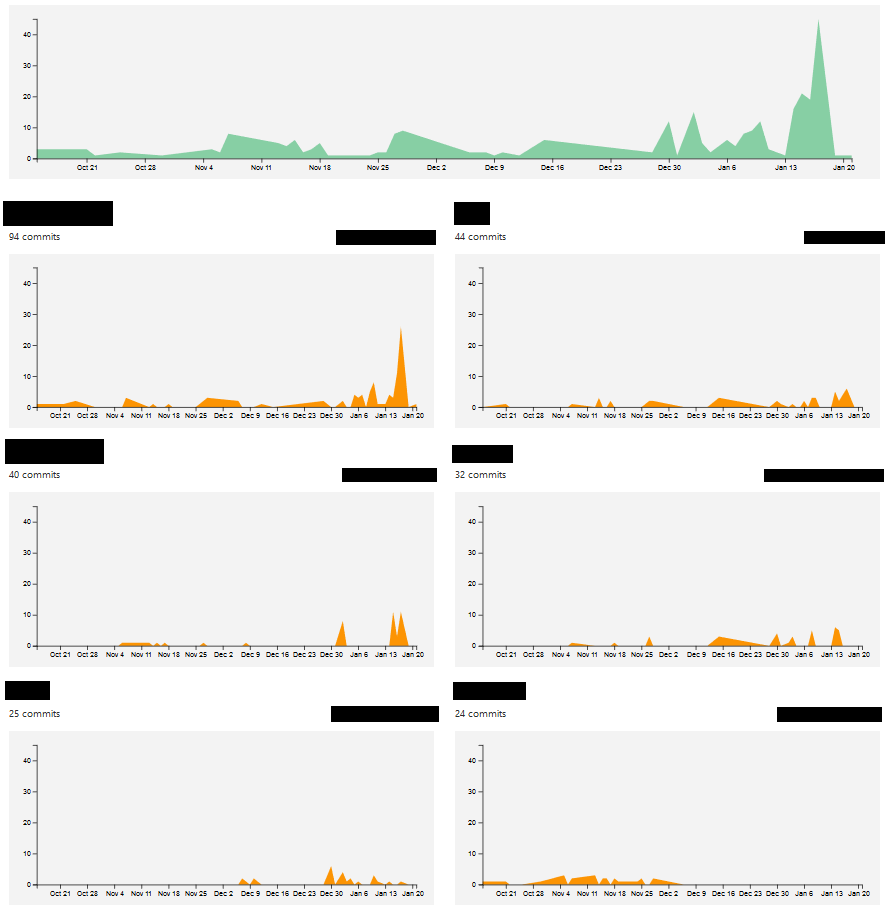
\includegraphics[width=.9\linewidth]{slike/aktivnost.PNG} %veličina u odnosu na širinu linije
			\caption{Primjer slike s potpisom 2}
			\label{fig:promjene2} %label mora biti drugaciji za svaku sliku
		\end{figure}
		
		Referenciranje slike \ref{fig:promjene2} u tekstu.
		
		\eject
		
	
	\chapter{Specifikacija programske potpore}
		
	\section{Funkcionalni zahtjevi}
			
			
			\noindent \textbf{Dionici:}
			
			\begin{packed_enum}
				
				\item Osoba koja izrađuje makete (administrator)
				\item Korisnici aplikacije		
				\item Razvojni tim
				
			\end{packed_enum}
			
			\noindent \textbf{Aktori i njihovi funkcionalni zahtjevi:}
			
			
			\begin{packed_enum}
				\item  \underbar{Neregistrirani korisnik (inicijator) može:}
				
				\begin{packed_enum}
					
					\item Vidjeti minijature (“thumbnailove”) objavljenih priča
					\item Kliknuti na priču i detaljnije pregledati sav sadržaj
					\item Komentirati priču
					\item Vidjeti broj pozitivnih i negativnih ocjena priče
					\item Registrirati se
					\item Pregledati minijature maketa dostupnih u webshopu
					\item Svaku maketu detaljno pregledati
					\item Kupiti maketu iz webshopa, pritom unoseći svoje podatke
					\item Kupiti jedinstvenu maketu iz priče, pritom unoseći svoje podatke
				\end{packed_enum}
			
				\item  \underbar{Registrirani korisnik (inicijator) može:}
				
				\begin{packed_enum}
					
					\item Sve što može i neregistrirani korisnik
					\item Predložiti temu administratoru kroz formular
					\item Predložiti priču administratoru kroz formular
					\item Ocijeniti priču
					\item Postaviti vlastitu profilnu sliku
					\item Gledati profilne stranice drugih korisnika
					\item Upravljati postavkama o privatnosti
					\item Uređivati vlastite podatke
					\item Obrisati vlastiti profil
					\item Kupiti maketu iz webshopa bez da unosi podatke
					\item Kupiti maketu iz priče bez da unosi podatke
					\item Ocijeniti maketu u webshopu
					\item Naručiti custom maketu kroz formular
					\item Prihvatiti ili odbiti cijenu za custom maketu

				\end{packed_enum}
							\item  \underbar{Administrator (inicijator) može:}
			
				\begin{packed_enum}
					
					\item Objaviti priču
					\item Pregledati predložene teme i priče
					\item Odgovoriti na predloženu temu
					\item Objaviti predloženu priču
					\item Komentirati priče
					\item Omogućiti prodaju jedinstvene makete iz priče
					\item Pregledati profile registriranih korisnika
					\item Vidjeti koji korisnik je kako ocijenio pojedinu priču
					\item Zabraniti pristup svakom pojedinom korisniku
					\item Uređivati makete u web trgovini
					\item Dodavati makete u web trgovinu
					\item Uklanjati makete iz web trgovine
					\item Pregledati zahtjeve za custom makete
					\item Ponuditi cijenu za zahtjev ili ga odbiti
					\item Pregledati povijest svih transakcija
					
				\end{packed_enum}
							\item  \underbar{Baza podataka (sudionik):}
		
				\begin{packed_enum}
					
					\item Pohranjuje podatke o korisnicima i administratoru
					\item Pohranjuje priče i komentare
					\item Pohranjuje podatke o maketama za prodaju
					\item Pohranjuje podatke o svim transakcijama
					
				\end{packed_enum}
			\end{packed_enum}
			
			\eject 
			
			
				
			\subsection{Obrasci uporabe}
				
				
			
				
					\noindent \underbar{\textbf{UC1 - Pregled priča}}
					\begin{packed_item}

						\item \textbf{Glavni sudionik: }Registrirani korisnik i neregistrirani korisnik
						\item  \textbf{Cilj:} Pregledati jednu ili više priča
						\item  \textbf{Sudionici:} Baza podataka
						\item  \textbf{Preduvjet:} Nema
						\item  \textbf{Opis osnovnog tijeka:}
						\item[] \begin{packed_enum}
							\item Pregled priče je prikazan kada se učita aplikacija
						\end{packed_enum}
		
					\end{packed_item}
				
					\noindent \underbar{\textbf{UC2 - Detaljan pregled priča}}
					\begin{packed_item}
						
						\item \textbf{Glavni sudionik: }Registrirani korisnik i neregistrirani korisnik
						\item  \textbf{Cilj:} Pregledati jednu priču detaljno, zajedno sa svim multimedijskim sadržajima koji su dio priče
						\item  \textbf{Sudionici:} Baza podataka
						\item  \textbf{Preduvjet:} Nema
						\item  \textbf{Opis osnovnog tijeka:}
						
						\item[] \begin{packed_enum}
							\item Korisnik odabire priču pritiskom na nju
							\item Priča je prikazana na zaslonu
						\end{packed_enum}
						
					\end{packed_item}
					\noindent \underbar{\textbf{UC3 - Komentiranje priče}}
					\begin{packed_item}
						
						\item \textbf{Glavni sudionik: }Registrirani korisnik i neregistrirani korisnik
						\item  \textbf{Cilj:} Ostaviti komentar na određenu priču
						\item  \textbf{Sudionici:} Baza podataka
						\item  \textbf{Preduvjet:} Nema
						\item  \textbf{Opis osnovnog tijeka:}
						
						\item[] \begin{packed_enum}
							\item Korisnik upiše svoj komentar u namijenjeni prostor
							\item Korisnik pritisne gumb za objavljivanje komentara
						\end{packed_enum}
						
					\end{packed_item}
				
					\noindent \underbar{\textbf{UC4 - Registracija korisnika}}
					\begin{packed_item}
						
						\item \textbf{Glavni sudionik: }Neregistrirani korisnik
						\item  \textbf{Cilj:} Unjeti korisnikove podatke u bazu podataka
						\item  \textbf{Sudionici:} Baza podataka
						\item  \textbf{Preduvjet:} Nema
						\item  \textbf{Opis osnovnog tijeka:}
						
						\item[] \begin{packed_enum}
							\item Korisnik unese svoje podatke
							\item Pritisne gumb za slanje podataka 
						\end{packed_enum}
						
					\end{packed_item}
				
					\noindent \underbar{\textbf{UC5 - Pregled maketa u webshopu}}
					\begin{packed_item}
						
						\item \textbf{Glavni sudionik: }Registrirani korisnik i neregistrirani korisnik
						\item  \textbf{Cilj:} Otvaranje pregleda maketa na stranici web trgovine
						\item  \textbf{Sudionici:} Baza podataka
						\item  \textbf{Preduvjet:} Nema
						\item  \textbf{Opis osnovnog tijeka:}
						
						\item[] \begin{packed_enum}
							
							\item Korisnik pritisne na poveznicu za otvaranje web trgovine
						\end{packed_enum}
						
					\end{packed_item}
						
					\noindent \underbar{\textbf{UC6 - Detaljni pregled makete u web trgovini}}
					\begin{packed_item}
						
						\item \textbf{Glavni sudionik: }Registrirani korisnik i neregistrirani korisnik
						\item  \textbf{Cilj:} Omogućuje detaljni pregled na maketu u web trgovini
						\item  \textbf{Sudionici:} Baza podataka
						\item  \textbf{Preduvjet:} Nema
						\item  \textbf{Opis osnovnog tijeka:}
						
						\item[] \begin{packed_enum}
							
							\item Korisnik odabire detaljan pregled makete
						\end{packed_enum}
						
					\end{packed_item}
				
					\noindent \underbar{\textbf{UC7 - Kupnja makete iz web trgovine}}
					\begin{packed_item}
						
						\item \textbf{Glavni sudionik: }Registrirani korisnik i neregistrirani korisnik
						\item  \textbf{Cilj:} Kupnja makete
						\item  \textbf{Sudionici:} Baza podataka
						\item  \textbf{Preduvjet:} Postojanje neprodane makete
						\item  \textbf{Opis osnovnog tijeka:}
						
						\item[] \begin{packed_enum}
							
							\item Korisnik dodaje maketu u košaricu
							\item Korisnik potvrđuje narudžbu
							\item Narudžba se prikazuje u listi aktivnih narudžbi administratora
						\end{packed_enum}
						
					\end{packed_item}
				
					\noindent \underbar{\textbf{UC8 - Kupnja makete iz priče}}
					\begin{packed_item}
						
						\item \textbf{Glavni sudionik: }Registrirani korisnik i neregistrirani korisnik
						\item  \textbf{Cilj:} Kupnja makete
						\item  \textbf{Sudionici:} Baza podataka
						\item  \textbf{Preduvjet:} Postojanje neprodane makete
						\item  \textbf{Opis osnovnog tijeka:}
						
						\item[] \begin{packed_enum}
							
							\item Korisnik dodaje maketu u košaricu
							\item Korisnik potvrđuje narudžbu
							\item Narudžba se prikazuje u listi aktivnih narudžbi administratora
						\end{packed_enum}
						
					\end{packed_item}
				
					\noindent \underbar{\textbf{UC9 - Unošenje podataka o kupnji}}
					\begin{packed_item}
						
						\item \textbf{Glavni sudionik: }Registrirani korisnik i neregistrirani korisnik
						\item  \textbf{Cilj:} Naručivanje makete
						\item  \textbf{Sudionici:} Baza podataka
						\item  \textbf{Preduvjet:} Odabir željenih proizvoda
						\item  \textbf{Opis osnovnog tijeka:}
						
						\item[] \begin{packed_enum}
							\item Korisnik odabire jednu ili više maketa koje želi kupiti
							\item Unosi osobne podatke u formular narudžbe
							\item Potvrđuje narudžbu
						\end{packed_enum}
						
					\end{packed_item}
				
					\noindent \underbar{\textbf{UC10 - Predlaganje teme administratoru}}
					\begin{packed_item}
						
						\item \textbf{Glavni sudionik: }Registrirani korisnik
						\item  \textbf{Cilj:} Predlaganje teme za priču
						\item  \textbf{Sudionici:} Baza podataka
						\item  \textbf{Preduvjet:} Nema
						\item  \textbf{Opis osnovnog tijeka:}
						
						\item[] \begin{packed_enum}
							\item Korisnik odabire opciju za predlaganje nove teme
							\item Korisnik popunjava obrazac za predlaganje teme
							\item Korisnik sprema promjene
							\item Baza podataka se ažurira
						\end{packed_enum}
						
					\end{packed_item}
				
					\noindent \underbar{\textbf{UC11 - Predlaganje priče administratoru}}
					\begin{packed_item}
						
						\item \textbf{Glavni sudionik: }Registrirani korisnik
						\item  \textbf{Cilj:} Predlaganje teme za priču
						\item  \textbf{Sudionici:} Baza podataka
						\item  \textbf{Preduvjet:} Nema
						\item  \textbf{Opis osnovnog tijeka:}
						
						\item[] \begin{packed_enum}
							\item Korisnik odabire opciju za predlaganje nove priče
							\item Korisnik popunjava obrazac za predlaganje priče
							\item Korisnik sprema promjene
							\item Baza podataka se ažurira
						\end{packed_enum}
						
					\end{packed_item}
				
					\noindent \underbar{\textbf{UC12 - Ocjenjivanje priče}}
					\begin{packed_item}
						\item \textbf{Glavni sudionik: }Registrirani korisnik
						\item  \textbf{Cilj:} Korisnik želi ocijeniti priču
						\item  \textbf{Sudionici:} Baza podataka
						\item  \textbf{Preduvjet:} Korisnik gleda priču
						\item  \textbf{Opis osnovnog tijeka:}
						
						\item[] \begin{packed_enum}
							\item Korisnik ocijenjuje priču pritiskom na gumb
						\end{packed_enum}
						
					\end{packed_item}
					
					\noindent \underbar{\textbf{UC13 - Naručivanje personalizirane makete}}
					\begin{packed_item}
						\item \textbf{Glavni sudionik: }Registrirani korisnik
						\item  \textbf{Cilj:} Zahtjev za personaliziranom maketom
						\item  \textbf{Sudionici:} Administrator, baza podataka
						\item  \textbf{Preduvjet:} Nema
						\item  \textbf{Opis osnovnog tijeka:}
						
						\item[] \begin{packed_enum}
							\item Korisnik pritišće gumb za slanje zahtjeva o personaliziranoj maketi
							\item Korisnik ispunjava formular o specifičnostima željene makete te prilaže svoje skice, slike i tekstualne opise
							\item Zahtjev se šalje administratoru na razmatranje
						\end{packed_enum}
						
					\end{packed_item}
				
					\noindent \underbar{\textbf{UC14 - Upravljanje vlastitim profilom}}
					\begin{packed_item}
						
						\item \textbf{Glavni sudionik: }Registrirani korisnik
						\item  \textbf{Cilj:} Urediti podatke profila
						\item  \textbf{Sudionici:} Baza podataka
						\item  \textbf{Preduvjet:} Nema
						\item  \textbf{Opis osnovnog tijeka:}
						
						\item[] \begin{packed_enum}
							\item Korisnik odlazi u postavke profila
							\item Mijenja podatke koje želi
							\item Potvrđuje izmjene
							\item Izmjene se pohranjuju u bazi podataka
							\item Korisniku se ažurira profil
						\end{packed_enum}
						
					\end{packed_item}
				
					\noindent \underbar{\textbf{UC15 - Objavljivanje priče}}
					\begin{packed_item}
						
						\item \textbf{Glavni sudionik: }Administrator
						\item  \textbf{Cilj:} Napisati i objaviti novu priču
						\item  \textbf{Sudionici:} Baza podataka
						\item  \textbf{Preduvjet:} Nema
						\item  \textbf{Opis osnovnog tijeka:}
						
						\item[] \begin{packed_enum}
							\item Korisnik odabire opciju za dodavanje priče
							\item Korisnik ispunjava obrazac
							\item Korisnik sprema promjene
							\item Baza podataka se ažurira
						\end{packed_enum}
					
						\item  \textbf{Opis mogućih odstupanja:}
						
						\item[] \begin{packed_item}
							
							\item[2.a] Korisnik ispunjava obrazac, ali ne odabere opciju “Spremi promjenu”
							\item[] \begin{packed_enum}
								
								\item Sustav obavještava korisnika da nije spremio podatke prije izlaska iz prozora
								
							\end{packed_enum}
							
						\end{packed_item}
				
						
					\end{packed_item}
				
					\noindent \underbar{\textbf{UC16 - Pregledavanje predloženih tema}}
					\begin{packed_item}
						
						\item \textbf{Glavni sudionik: }Administrator
						\item  \textbf{Cilj:} Pregledati predložene teme
						\item  \textbf{Sudionici:} Baza podataka
						\item  \textbf{Preduvjet:} Nema
						\item  \textbf{Opis osnovnog tijeka:}
						
						\item[] \begin{packed_enum}
							
							\item Otvoriti pregled predloženih tema 
						\end{packed_enum}
						
					\end{packed_item}
				
					\noindent \underbar{\textbf{UC17 - Pregledavanje predloženih priča}}
					\begin{packed_item}
						
						\item \textbf{Glavni sudionik: }Administrator
						\item  \textbf{Cilj:} Pregledati predloženu priču
						\item  \textbf{Sudionici:} Baza podataka
						\item  \textbf{Preduvjet:} Nema
						\item  \textbf{Opis osnovnog tijeka:} 
						
						\item[] \begin{packed_enum}
							
							\item Otvoriti pregled predloženih priča
						\end{packed_enum}
						
					\end{packed_item}
				
					\noindent \underbar{\textbf{UC18 - Odgovor na predloženu temu}}
					\begin{packed_item}
						
						\item \textbf{Glavni sudionik: }Administrator
						\item  \textbf{Cilj:} Prihvatiti ili odbiti predloženu temu
						\item  \textbf{Sudionici:} Baza podataka
						\item  \textbf{Preduvjet:} Nema
						\item  \textbf{Opis osnovnog tijeka:}
						
						\item[] \begin{packed_enum}
							
							\item Stisnuti gumb prihvati ili odbij
						\end{packed_enum}
						
					\end{packed_item}
				
					\noindent \underbar{\textbf{UC19 - Objavljivanje predložene priče}}
					\begin{packed_item}
						
						\item \textbf{Glavni sudionik: }Administrator
						\item  \textbf{Cilj:} Objavljivanje predložene priče
						\item  \textbf{Sudionici:} Baza podataka
						\item  \textbf{Preduvjet:} Nema
						\item  \textbf{Opis osnovnog tijeka:}
						
						\item[] \begin{packed_enum}
							
							\item Administrator pregledava predložene priče
							\item Administrator objavljuje priču
						\end{packed_enum}
						
					\end{packed_item}
				
					\noindent \underbar{\textbf{UC20 - Pregled košarice}}
					\begin{packed_item}
						
						\item \textbf{Glavni sudionik: }Administrator, registrirani i neregistrirani korisnik
						\item  \textbf{Cilj:} Pregledati proizvode košarice
						\item  \textbf{Sudionici:} Baza podataka
						\item  \textbf{Preduvjet:} Nema
						\item  \textbf{Opis osnovnog tijeka:}
						
						\item[] \begin{packed_enum}
							
							\item Korisnik bira opciju pregleda košarice
							\item Korisnik dobiva pregled proizvoda u košarici
							\item Korisnik ima opciju pokretanja kupnje 
						\end{packed_enum}
						
					\end{packed_item}
				
					\noindent \underbar{\textbf{UC21 - Omogućavanje prodaje jednistvene makete iz priče}}
					\begin{packed_item}
						
						\item \textbf{Glavni sudionik: }Administrator
						\item  \textbf{Cilj:} Pružiti korisnicima mogućnost kupnje jedinstvenih maketa koje je napravio administrator
						\item  \textbf{Sudionici:} Baza podataka
						\item  \textbf{Preduvjet:} Kreirana je priča i u priči se radi o novoj maketi
						\item  \textbf{Opis osnovnog tijeka:}
						
						\item[] \begin{packed_enum}
							
							\item Administrator odabire opciju dodavanja cijene
							\item Administrator definira cijenu i specifikacije makete
							\item Administrator potvrđuje svoj odabir
							\item Prikazuje se opcija za kupnju na dnu priče
						\end{packed_enum}
						\item  \textbf{Opis mogućih odstupanja:}
					
						\item[] \begin{packed_item}
							
							\item[2.a] Administrator odustaje od definiranja cijene
							
							\item[] \begin{packed_enum}
								
								\item Ne spremaju se promjene i administrator se vraća na pregled cijele priče
								
							\end{packed_enum}
							
						\end{packed_item}
					\end{packed_item}
				
					\noindent \underbar{\textbf{UC22 - Uređivanje vlastitih podataka}}
					\begin{packed_item}
						
						\item \textbf{Glavni sudionik: } Registrirani korisnik
						\item  \textbf{Cilj:} Korisnik mijenja ili dodaje vlastite podatke
						\item  \textbf{Sudionici:} Baza podataka
						\item  \textbf{Preduvjet:} Nema
						\item  \textbf{Opis osnovnog tijeka:}
						
						\item[] \begin{packed_enum}
							
							\item Korisnik mijenja ili dodaje svoje podatke
							\item Korisnik potvrđuje promjenu podataka
							\item Korisnik upisuje lozinku
						\end{packed_enum}
						
					\end{packed_item}
			
					\noindent \underbar{\textbf{UC23 - Upravljanje postavkama o privatnosti}}
					\begin{packed_item}
						
						\item \textbf{Glavni sudionik: } Registrirani korisnik
						\item  \textbf{Cilj:} Personaliziranje postavki privatnosti
						\item  \textbf{Sudionici:} Baza podataka
						\item  \textbf{Preduvjet:} Nema
						\item  \textbf{Opis osnovnog tijeka:}
						
						\item[] \begin{packed_enum}
							
							\item Korisnik se registrira u svoj profil
							\item U postavkama mijenja željene postavke privatnosti
							\item Potvrđuje željene izmjene
							\item Izmjene se spremaju u bazu podataka
							\item Ažurira se korisnikov profil
						\end{packed_enum}
						
					\end{packed_item}
				
				
					\noindent \underbar{\textbf{UC24 - Promjena profilne slike}}
					\begin{packed_item}
						
						\item \textbf{Glavni sudionik: } Registrirani korisnik
						\item  \textbf{Cilj:} Promijeniti sliku profila
						\item  \textbf{Sudionici:} Baza podataka
						\item  \textbf{Preduvjet:} Nema
						\item  \textbf{Opis osnovnog tijeka:}
						
						\item[] \begin{packed_enum}
							
							\item Korisnik odabere opciju promjene profila
							\item Korisnik mijenja sliku profila
							\item Korisnik sprema promjenu
							\item Baza podataka se ažurira
						\end{packed_enum}
						
					\end{packed_item}
				
					\noindent \underbar{\textbf{UC25 - Brisanje vlastitog profila}}
					\begin{packed_item}
						
						\item \textbf{Glavni sudionik: } Registrirani korisnik
						\item  \textbf{Cilj:} Brisanje korisnikovih podataka iz sustava
						\item  \textbf{Sudionici:} Baza podataka
						\item  \textbf{Preduvjet:} Nema
						\item  \textbf{Opis osnovnog tijeka:}
						
						\item[] \begin{packed_enum}
							
							\item Korisnik odabire opciju brisanja svojeg profila
							\item Korisnikovi se podatci brišu iz baze podataka
							\item Korisnik u komentarima postaje vidljiv kao anonimni korisnik
						\end{packed_enum}
						
					\end{packed_item}
					
					
					\noindent \underbar{\textbf{UC26 - Uređivanje makete u web trgovini}}
					\begin{packed_item}
						
						\item \textbf{Glavni sudionik: } Administrator
						\item  \textbf{Cilj:} Izmjena podataka o maketi
						\item  \textbf{Sudionici:} Baza podataka
						\item  \textbf{Preduvjet:} Nema
						\item  \textbf{Opis osnovnog tijeka:}
						
						\item[] \begin{packed_enum}
							
							\item Administrator odabire opciju za uređivanje
							\item Administrator odabire specifikacije koje treba promijeniti
							\item Promjena se pohranjuje u bazu podataka
							\item Promjena postaje vidljiva na web trgovini
						\end{packed_enum}
						\item  \textbf{Opis mogućih odstupanja:}
						
						\item[] \begin{packed_item}
							
							\item[2.a] Administrator nije odabrao spremi opciju
							
							\item[] \begin{packed_enum}
								
								\item Poruka upozorenja da uređeni podaci nisu spremljeni
								
							\end{packed_enum}
							
						\end{packed_item}
					\end{packed_item}
				
					\noindent \underbar{\textbf{UC27 - Dodavanje makete u web trgovinu}}
					\begin{packed_item}
						
						\item \textbf{Glavni sudionik: } Administrator
						\item  \textbf{Cilj:} Dodati maketu u trgovinu
						\item  \textbf{Sudionici:} Baza podataka
						\item  \textbf{Preduvjet:} Nema
						\item  \textbf{Opis osnovnog tijeka:}
						
						\item[] \begin{packed_enum}
							
							\item Odabir opcije za dodavanje makete u web trgovinu
							\item Maketa dostupna u web trgovini za kupnju
						\end{packed_enum}
						
					\end{packed_item}
				
					\noindent \underbar{\textbf{UC28 - Uklanjanje makete iz web trgovine}}
					\begin{packed_item}
						
						\item \textbf{Glavni sudionik: } Administrator
						\item  \textbf{Cilj:} Uklanjanje makete iz web trgovina
						\item  \textbf{Sudionici:} Baza podataka
						\item  \textbf{Preduvjet:} Nema
						\item  \textbf{Opis osnovnog tijeka:}
						
						\item[] \begin{packed_enum}
							
							\item Administrator pregledava makete u web trgovini
							\item Administrator uklanja maketu iz web trgovine
						\end{packed_enum}
						
					\end{packed_item}
				
				
				
					\noindent \underbar{\textbf{UC29 - Ocjenjivanje makete u web trgovini}}
					\begin{packed_item}
						
						\item \textbf{Glavni sudionik: } Registrirani korisnik
						\item  \textbf{Cilj:} Ocjeniti maketu
						\item  \textbf{Sudionici:} Baza podataka
						\item  \textbf{Preduvjet:} Postojanje makete
						\item  \textbf{Opis osnovnog tijeka:}
						
						\item[] \begin{packed_enum}
							\item Odabrati ocjenu pritiskom na nju
						\end{packed_enum}
						
					\end{packed_item}
				
					\noindent \underbar{\textbf{UC30 - Naručivanje personalizirane makete ispunjavanjem formulara}}
					\begin{packed_item}
						
						\item \textbf{Glavni sudionik: } Registrirani korisnik i neregistrirani korisnik
						\item  \textbf{Cilj:} Naručiti maketu
						\item  \textbf{Sudionici:} Baza podataka
						\item  \textbf{Preduvjet:} Maketa na zalihi u web trgovini
						
						\item  \textbf{Opis osnovnog tijeka:}
						
						\item[] \begin{packed_enum}
							
							\item Ispunjavanje formulara
							\item Slanje formulara pritiskom na gumb
						\end{packed_enum}
						
					\end{packed_item}
				
					\noindent \underbar{\textbf{UC31 - Pregled profila registriranih korisnika}}
					\begin{packed_item}
						
						\item \textbf{Glavni sudionik: } Registrirani i neregistriran korisnik
						\item  \textbf{Cilj:} Pregledati profil registriranog korisnika
						\item  \textbf{Sudionici:} Baza podataka
						\item  \textbf{Preduvjet:} Postojanje profila koji želimo pregledati
						\item  \textbf{Opis osnovnog tijeka:}
						
						\item[] \begin{packed_enum}
							\item Pritisak na gumb pregled profila
						\end{packed_enum}
						
					\end{packed_item}
				
					\noindent \underbar{\textbf{UC32 - Pregled ocjena}}
					\begin{packed_item}
						
						\item \textbf{Glavni sudionik: } Administrator
						\item  \textbf{Cilj:} Pregledati ocjene
						\item  \textbf{Sudionici:} Baza podataka
						\item  \textbf{Preduvjet:} Nema
						\item  \textbf{Opis osnovnog tijeka:}
						
						\item[] \begin{packed_enum}
							\item Odabrati opciju za pregled ocjena
						\end{packed_enum}
						
					\end{packed_item}
				
					\noindent \underbar{\textbf{UC33 - Moderiranje pristupa korisnicima}}
					\begin{packed_item}
						
						\item \textbf{Glavni sudionik: } Administrator
						\item  \textbf{Cilj:} Moderirati pristup korisnicima
						\item  \textbf{Sudionici:} Baza podataka
						\item  \textbf{Preduvjet:} Nema
						\item  \textbf{Opis osnovnog tijeka:}
						
						\item[] \begin{packed_enum}
							
							\item Odabrati opciju za upravljanje postavkama pristupa korisnika
						\end{packed_enum}
						
					\end{packed_item}
				
					\noindent \underbar{\textbf{UC34 - Predlaganje sadržaja}}
					\begin{packed_item}
						
						\item \textbf{Glavni sudionik: } Registrirani korisnik
						\item  \textbf{Cilj:} Predložiti sadržaj administratoru
						\item  \textbf{Sudionici:} Baza podataka
						\item  \textbf{Preduvjet:} Nema
						\item  \textbf{Opis osnovnog tijeka:}
						
						\item[] \begin{packed_enum}
							
							\item Odabir opcije predlaganja sadržaja
							\item Nudi se opcija predlaganja teme ili priče
						\end{packed_enum}
						
					\end{packed_item}
				
					\noindent \underbar{\textbf{UC35 - Pregled zahtjeva za personaliziranom maketom}}
					\begin{packed_item}
						
						\item \textbf{Glavni sudionik: } Administrator
						\item  \textbf{Cilj:} Administrator gleda korisnikov zahjev za personaliziranom maketom
						\item  \textbf{Sudionici:} Baza podataka
						\item  \textbf{Preduvjet:} Postavljen zahtjev za personaliziranu maketu
						\item  \textbf{Opis osnovnog tijeka:}
						
						\item[] \begin{packed_enum}
							\item Administrator gleda na postavljen zahtjev
						\end{packed_enum}
						
					\end{packed_item}
				
					\noindent \underbar{\textbf{UC36 - Odluka o zahtjevu za personaliziranom maketom}}
					\begin{packed_item}
						
						\item \textbf{Glavni sudionik: } Administrator
						\item  \textbf{Cilj:} Administrator potvrđuje ili odbija zahtjev o personaliziranoj maketi
						\item  \textbf{Sudionici:} Baza podataka
						\item  \textbf{Preduvjet:} Postavljen zahtjev za personaliziranu maketu
						\item  \textbf{Opis osnovnog tijeka:}
						
						\item[] \begin{packed_enum}
							\item Administrator upisuje ponuđenu cijenu za maketu
							\item Administrator šalje odluku
						\end{packed_enum}
						
					\end{packed_item}
				
					\noindent \underbar{\textbf{UC37 - Pregled povijesti transakcija}}
					\begin{packed_item}
						
						\item \textbf{Glavni sudionik: } Administrator
						\item  \textbf{Cilj:} Uvid u povijest svih transakcija
						\item  \textbf{Sudionici:} Baza podataka
						\item  \textbf{Preduvjet:} Nema
						\item  \textbf{Opis osnovnog tijeka:}
						
						\item[] \begin{packed_enum}
							
							\item Administrator bira pregled povijesti transakcija
							\item Dohvaćaju se podaci iz baze podataka
							\item Prikazuju se podaci o transakcijama
						\end{packed_enum}
						
					\end{packed_item}
				
					\noindent \underbar{\textbf{UC38 - Prihvaćanje ili odbijanje cijene za personaliziranu maketu}}
					\begin{packed_item}
						
						\item \textbf{Glavni sudionik: } Registrirani korisnik
						\item  \textbf{Cilj:} Davanje povratne informacije administratoru je li prihvaćena njegova cijena ili ne
						\item  \textbf{Sudionici:} Baza podataka
						\item  \textbf{Preduvjet:} Inicijaliziran je postupak naručivanja custom makete, korisnik je poslao skicu, a administrator je kreirao cijenu
						\item  \textbf{Opis osnovnog tijeka:}
						
						\item[] \begin{packed_enum}
							
							\item Korisnik otvara sučelje za komunikaciju s administratorom
							\item Korisnik prihvaća ili odbija ponuđenu cijenu
							\item Administratoru dolazi potvrda o odbijanju ili potvrđivanju ponuđene cijene
							\item Administrator šalje maketu korisniku
						\end{packed_enum}
						
					\end{packed_item}
				
				
				\subsubsection{Dijagrami obrazaca uporabe}
					
					\begin{figure}
						\centering
						\includegraphics[scale=0.34]{"slike/Funkcionalnost neregistriranog korisnika"}
						\caption{Dijagram obrasca uporabe funkcionalnosti neregistriranog korisnika}
						\label{fig:funkcionalnost-neregistriranog-korisnika}   
					\end{figure}
					
					\begin{figure}
						\centering
						\includegraphics[scale=0.34]{"slike/Funkcionalnost registriranog korisnika"}
						\caption{Dijagram obrasca uporabe funkcionalnosti registriranog korisnika}
						\label{fig:funkcionalnost-registriranog-korisnika}
					\end{figure}
					
					\begin{figure}
						\centering
						\includegraphics[scale=0.34]{"slike/Funkcionalnost administratora"}
						\caption{Dijagram obrasca uporabe funkcionalnosti administratora}
						\label{fig:funkcionalnost-administratora}
					\end{figure}
					
					
				\eject		
				
			\subsection{Sekvencijski dijagrami}
				
				\textbf{\textit{dio 1. revizije}}\\
				
				\textit{Nacrtati sekvencijske dijagrame koji modeliraju najvažnije dijelove sustava (max. 4 dijagrama). Ukoliko postoji nedoumica oko odabira, razjasniti s asistentom. Uz svaki dijagram napisati detaljni opis dijagrama.}
				\eject
	
		\section{Ostali zahtjevi}
		
		\begin{packed_item}
			
			\item  Sustav treba biti jednostavan za korištenje
			\item  Sustav treba biti implementiran kao web-aplikacija pomoću objektno-orijentiranih jezika
			\item  Sustav treba zadržati svoju funkcionalnost i prilikom neispravnog korištenja korisničkog sučelja
			\item  Sustav treba biti moguće nadograditi bez da se naruše postojeće funkcionalnosti
			\item  Sustav treba omogućiti rad više korisnika u stvarnom vremenu
			\item  Sutsav i korisničko sučelje trebaju podržavati dijakritičke znakove hrvatske abecede pri unosu i prikazu tekstualnog sadžaja
			\item  Sustav kao valutu koristi HRK
			\item  Sustavu se treba moći pristupiti iz javne mreže pomoću HTTPS
			\item  Veza s bazom podataka mora biti brza i kvalitetno zaštićena
			
		\end{packed_item}
			
			 
			 
			 
	
	\chapter{Arhitektura i dizajn sustava}
		
		%\textbf{\textit{dio 1. revizije}}\\

		%\textit{ Potrebno je opisati stil arhitekture te identificirati: podsustave, preslikavanje na radnu platformu, spremišta podataka, mrežne protokole, globalni upravljački tok i sklopovsko-programske zahtjeve. Po točkama razraditi i popratiti odgovarajućim skicama:}
	%\begin{itemize}
	%	\item 	\textit{izbor arhitekture temeljem principa oblikovanja pokazanih na predavanjima (objasniti zašto ste baš odabrali takvu arhitekturu)}
		%\item 	\textit{organizaciju sustava s najviše razine apstrakcije (npr. klijent-poslužitelj, baza podataka, datotečni sustav, grafičko sučelje)}
	%	\item 	\textit{organizaciju aplikacije (npr. slojevi frontend i backend, MVC arhitektura) }		
%	\end{itemize}

		Arhitektura našeg sustava dijeli se na tri podsustava: baza podataka, web aplikacija i web poslužitelj.
			
		\underbar{Web preglednik} program je koji služi kao posrednik između korisnika i web poslužitelja. Korisniku omogućuje pregled web-stranica te multimedijskih sadržaja vezanih uz njih. Svaka stranica pisana je u nekom kodu koji prosječnom korisniku ništa ne znači, no kako je svaki internetski preglednik ujedno i prevoditelj, on prikazuje stranicu u obliku koja je svakome razumljiva. Na taj način korisnik šalje zahtjeve web poslužitelju.
		
		\underbar{Web poslužitelj} kao osnovnu zadaću ima ostvarivanje komunikacije između klijenta i aplikacije.  Ta komunikacija ostvarena je HTTP-om (engl. HyperText Transfer Protocol). Upravo je web poslužitelj temelj rada web aplikacije. On ju pokreće i prosljeđuje zahtjeve zaprimljene od web preglednika.
		
		\underbar{Web aplikacija} koju korisnik koristi obrađuje njegove zahtjeve. Ukoliko je potrebno za obradu zahtjeva, web aplikacija komunicira s poslužiteljem baze podataka koji joj dohvaća i prosljeđuje potrebne podatke. Potom web aplikacija vraća odgovor u obliku HTML dokumenta te web preglednik to prikazuje korisniku u odgovarajućem formatu.
		
		Za izradu naše web aplikacije odlučili smo se za programski jezik Python s njegovim radnim okvirom Django. Koristili smo Bootstrap, HTML, CSS i JavaScript za prikaz web-stranica. Baza podataka implementirana je kroz PostgreSQL. Arhitektura sustava temeljit će se na MVT (eng. \textit{Model View Template}) obrascu koji se tek marginalno razlikuje od MVC (eng. \textit{Model View Controller}) obrasca. S obzirom da je MVT koncept podržan od strane Djanga, na raspolaganju su nam gotovi predlošci te nam znatno olakšavaju razvoj web aplikacije.
	
		Zahvaljujući nezavisnosti razvoja pojedinih djelova aplikacije možemo jednostavnije ispitivati i razvijati sustav, kao i dodavati nova svojstva. Kao što se može pretpostaviti, MVT koncept sastoji se od triju komponenti. "Model" i "View" na strani su poslužitelja i nisu vidljivi korisniku, dok je "Template" vidljiv na korisničkoj strani. "Model" je središnja jkomponenta sustava te pristupa bazi podataka. Pravilno formatira podatke dobivene od strane "View"-a te ih prosljeđuje bazi podataka i obrnuto. "View" prima podatke i zahtjeve kao što su "POST" i "GET" s klijentske strane. Također pravilno formatira primljene podatke te komunicira s druge dvije komponente MVT koncepta. "Template" služi za prikazivanje sadržaja na web-stranici. Sadrži statičke i dinamičke definicije prikaza sadržaja.
		
		\begin{figure} [!h] %ovaj [!h] je potreban za fiksiranje slike točno na ovo mjesto u pdf-u.
			\centering
			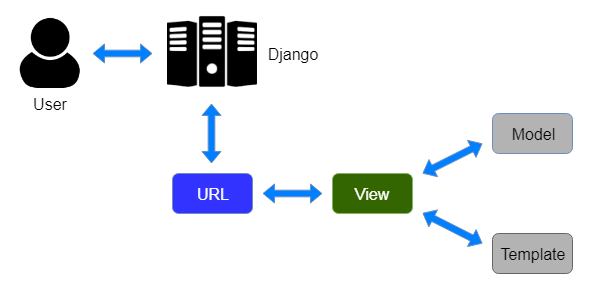
\includegraphics[width=0.7\linewidth]{slike/MVT}
			\caption{MVT koncept}
			\label{fig:mvt}
		\end{figure}
		
		\eject		

				
		\section{Baza podataka}
			
		Koristimo relacijsku bazu podataka napisanu u jeziku SQL te je ostvarujemo kroz postgreSQL. Pregled cijele baze imamo preko programa pgAdmin 4. Tamo gledamo spremaju li se promjene, jesu li one smislene te dodajemo specifičan sadržaj za testiranje. Django preko komponente "Model" pristupa bazi te je ona strukturno cijela sadržana u datoteci models.py.
		
			\subsection{Opis tablica}
			
				
				\begin{longtabu} to \textwidth {|X[10, l]|X[6, l]|X[20, l]|}
					
					\hline \multicolumn{3}{|c|}{\textbf{Korisnik}}	 \\[3pt] \hline
					\endfirsthead
					
					\hline \multicolumn{3}{|c|}{\textbf{Korisnik}}	 \\[3pt] \hline
					\endhead
					
					\hline 
					\endlastfoot
					
					\cellcolor{LightGreen}korisnikid & INT	&  	Redni broj korisnika (primarni ključ). 	\\ \hline
					email	& VARCHAR &  Korisnikov e-mail  (maksimalno 100 znakova). \\ \hline
					korisnickoime & VARCHAR & Ime koje predstavlja korisnika na stranici (maksimalno 20 znakova). \\ \hline 
					lozinka & VARCHAR & Korisnikova lozinka za prijavu (maksimalno 20 znakova).  \\ \hline 
					razinaautoriteta & INT & Razina autoriteta korisnika. 1 predstavlja korisnika, a 2 admina. \\ \hline 
					adresa & VARCHAR & Korisnikova adresa (maksimalno 100 znakova). \\ \hline 
					rodendan & DATE & Datum korisnikovog rođendana.  \\ \hline 
					datumregistracije & DATE & Datum korisnikove registracije.  \\ \hline 
					adresaprivatna & BOOL & Želi li korisnik javno prikazati svoju adresu na svome profilu? \\ \hline 
					rodendanprivatan & BOOL & Želi li korisnik javno prikazati svoj rođendan na svome profilu?   \\ \hline
					datumregistracije
					privatan & BOOL & Želi li korisnik javno prikazati svoj datum registracije na svome profilu?  \\ \hline 
					ime & VARCHAR &  Korisnikovo ime (maksimalno 50 znakova).  \\ \hline 
					prezime  & VARCHAR & Korisnikovo prezime (maksimalno 50 znakova).  \\ \hline 
					dozvoljenpristup & BOOL & Ima li korisnik dozvoljen pristup stranici?  \\ \hline 
					brojracuna & VARCHAR & Broj bankovnog računa korisnika. (21 znak)  \\ \hline
					\cellcolor{LightBlue} 
					profilnaid & INT & Redni broj medijske datoteke koja sadrži korisnikovu profilnu fotografiju. (strani ključ)  \\ \hline 
					emailprivatan & BOOL & Želi li korisnik javno prikazati svoj e-mail na svome profilu?   \\ \hline 
					imeprezimeprivatno & BOOL & Želi li korisnik javno prikazati svoje ime i prezime na svome profilu?  \\ \hline 					
					
				\end{longtabu}
			
				\begin{longtabu} to \textwidth {|X[10, l]|X[6, l]|X[20, l]|}
				
				\hline \multicolumn{3}{|c|}{\textbf{Komentar}}	 \\[3pt] \hline
				\endfirsthead
				
				\hline \multicolumn{3}{|c|}{\textbf{Komentar}}	 \\[3pt] \hline
				\endhead
				
				\hline 
				\endlastfoot
				
				\cellcolor{LightGreen}komentarid & INT	&  	Redni broj komentara (primarni ključ). 	\\ \hline
				sadrzaj	& VARCHAR &  Tekstualni sadržaj komentara (maksimalno 300 znakova). \\ \hline
				\cellcolor{LightGreen}
				korisnikid & INT & Redni broj korisnika koji je ostavio komentar. (strani ključ) \\ \hline 
				\cellcolor{LightBlue}
				pricaid & INT & Redni broj priče na kojoj je ostavljen komentar. (strani ključ) \\ \hline 	
				
				\end{longtabu}
			
				\begin{longtabu} to \textwidth {|X[10, l]|X[6, l]|X[20, l]|}
					
				\hline \multicolumn{3}{|c|}{\textbf{KorisnikDislajkaopricu}}	 \\[3pt] \hline
				\endfirsthead
				
				\hline \multicolumn{3}{|c|}{\textbf{KorisnikDislajkaopricu}}	 \\[3pt] \hline
				\endhead
				
				\hline 
				\endlastfoot
				
				\cellcolor{LightBlue}
				korisnikid & INT & Redni broj korisnika koji je označio sa "ne sviđa mi se". (strani ključ) \\ \hline 
				\cellcolor{LightBlue}
				pricaid & INT & Redni broj priče koja je označena sa "ne sviđa mi se". (strani ključ) \\ \hline 	
					
				\end{longtabu}
			
				\begin{longtabu} to \textwidth {|X[10, l]|X[6, l]|X[20, l]|}
					
					\hline \multicolumn{3}{|c|}{\textbf{KorisnikLajkaopricu}}	 \\[3pt] \hline
					\endfirsthead
					
					\hline \multicolumn{3}{|c|}{\textbf{KorisnikLajkaopricu}}	 \\[3pt] \hline
					\endhead
					
					\hline 
					\endlastfoot
					
					\cellcolor{LightBlue}
					korisnikid & INT & Redni broj korisnika koji je označio priču sa "sviđa mi se". (strani ključ) \\ \hline 
					\cellcolor{LightBlue}
					pricaid & INT & Redni broj priče koja je označena sa "sviđa mi se". (strani ključ) \\ \hline 	
					
				\end{longtabu}
			
			\begin{longtabu} to \textwidth {|X[10, l]|X[6, l]|X[20, l]|}
				
				\hline \multicolumn{3}{|c|}{\textbf{Maketa}}	 \\[3pt] \hline
				\endfirsthead
				
				\hline \multicolumn{3}{|c|}{\textbf{Maketa}}	 \\[3pt] \hline
				\endhead
				
				\hline 
				\endlastfoot
				
				\cellcolor{LightGreen}maketaid & INT	&  	Redni broj makete (primarni ključ). 	\\ \hline
				\cellcolor{LightBlue}
				dimenzije & VARCHAR & Dimenzije makete u centimetrima. \\ \hline 
				\cellcolor{LightBlue}
				mediaid & INT & Redni broj medijske datoteke koja sadrži sliku makete. (strani ključ) \\ \hline 	
				
			\end{longtabu}
		
			\begin{longtabu} to \textwidth {|X[10, l]|X[6, l]|X[20, l]|}
				
				\hline \multicolumn{3}{|c|}{\textbf{MaketaKupljena}}	 \\[3pt] \hline
				\endfirsthead
				
				\hline \multicolumn{3}{|c|}{\textbf{MaketaKupljena}}	 \\[3pt] \hline
				\endhead
				
				\hline 
				\endlastfoot
				
				\cellcolor{LightGreen}id & INT	&  	Redni broj kupovine makete (primarni ključ). 	\\      \hline			
				kolicina & INT & Broj istih maketa kupljenih pri ovoj narudžbi. \\ \hline 
				\cellcolor{LightBlue}
				maketaid & INT & Redni broj navedene makete. (strani ključ) \\ \hline 
				\cellcolor{LightBlue}
				materijalid & INT & Redni broj materijala od kojeg je izgrađena navedena maketa. (strani ključ) \\ \hline 	
				\cellcolor{LightBlue}
				maketaid & INT & Redni broj transakcije u pitanju. (strani ključ) \\ \hline 
				
			\end{longtabu}
		
			\begin{longtabu} to \textwidth {|X[10, l]|X[6, l]|X[20, l]|}
				
				\hline \multicolumn{3}{|c|}{\textbf{Materijal}}	 \\[3pt] \hline
				\endfirsthead
				
				\hline \multicolumn{3}{|c|}{\textbf{Materijal}}	 \\[3pt] \hline
				\endhead
				
				\hline 
				\endlastfoot
				
				\cellcolor{LightGreen}materijalid & INT	&  	Redni broj materijala (primarni ključ). 	\\      \hline			
				ime & VARCHAR & Ime materijala (maksimalno 100 znakova). \\ \hline 
				
			\end{longtabu}
		
			\begin{longtabu} to \textwidth {|X[10, l]|X[6, l]|X[20, l]|}
			
			\hline \multicolumn{3}{|c|}{\textbf{Media}}	 \\[3pt] \hline
			\endfirsthead
			
			\hline \multicolumn{3}{|c|}{\textbf{Media}}	 \\[3pt] \hline
			\endhead
			
			\hline 
			\endlastfoot
			
			\cellcolor{LightGreen}mediaid & INT	&  	Redni broj medijske datoteke (primarni ključ). 	\\      \hline			
			putdodatoteke & VARCHAR & Relativni put do datoteke u repozitoriju. \\ \hline 
			
			\end{longtabu}
				
				\begin{longtabu} to \textwidth {|X[10, l]|X[6, l]|X[20, l]|}
				
				\hline \multicolumn{3}{|c|}{\textbf{MultimedijaPriče}}	 \\[3pt] \hline
				\endfirsthead
				
				\hline \multicolumn{3}{|c|}{\textbf{MultimedijaPriče}}	 \\[3pt] \hline
				\endhead
				
				\hline 
				\endlastfoot
						
				poredakuprici & INT & Broj u poretku po kojem se slaže multimedija u nekoj priči. \\ \hline 
				\cellcolor{LightBlue}
				mediaid & INT & Redni broj medijske datoteke u pitanju. (strani ključ) \\ \hline 
				\cellcolor{LightBlue}
				pricaid & INT & Redni broj priče u pitanju. (strani ključ) \\ \hline 
				
			\end{longtabu}
		
		\begin{longtabu} to \textwidth {|X[10, l]|X[6, l]|X[20, l]|}
			
			\hline \multicolumn{3}{|c|}{\textbf{NapravljenaOd}}	 \\[3pt] \hline
			\endfirsthead
			
			\hline \multicolumn{3}{|c|}{\textbf{NapravljenaOd}}	 \\[3pt] \hline
			\endhead
			
			\hline 
			\endlastfoot
						
			cijena & FLOAT & Cijena makete napravljene od specifičnog materijala. \\ \hline 
			\cellcolor{LightBlue}
			maketaid & INT & Redni broj makete u pitanju. (strani ključ) \\ \hline 
			\cellcolor{LightBlue}
			materijalid & INT & Redni broj materijala u pitanju. (strani ključ) \\ \hline 
			
		\end{longtabu}
	
			\begin{longtabu} to \textwidth {|X[10, l]|X[6, l]|X[20, l]|}
				
				\hline \multicolumn{3}{|c|}{\textbf{Priča}}	 \\[3pt] \hline
				\endfirsthead
				
				\hline \multicolumn{3}{|c|}{\textbf{Priča}}	 \\[3pt] \hline
				\endhead
				
				\hline 
				\endlastfoot
				
				\cellcolor{LightGreen}pricaid & INT	&  	Redni broj priče (primarni ključ). 	\\      \hline			
				naslovprice & VARCHAR & Naslov priče (maksimalno 100 znakova). \\ \hline 
				datumprice & DATE & Datum objave priče. \\ \hline
				objavljena & BOOL & Je li priča objavljena? \\ \hline 
				maketaprodana & BOOL & Je li maketa iz priče (ako priča sadrži maketu) prodana? \\ \hline 
				\cellcolor{LightBlue}
				maketaid & INT & Redni broj makete u pitanju. (strani ključ) \\ \hline 
				\cellcolor{LightBlue}
				autorid & INT & Redni broj autora priču. (strani ključ) \\ \hline 
				\cellcolor{LightBlue}
				predloziopricuid & INT & Redni broj osobe koja je predložila priču. (strani ključ) \\ \hline 
				\cellcolor{LightBlue}
				tekstpriceid & INT & Redni broj medijske datoteke koja sadrži tekst priče. (strani ključ) \\ \hline 
				
			\end{longtabu}
		
			\begin{longtabu} to \textwidth {|X[10, l]|X[6, l]|X[20, l]|}
			
			\hline \multicolumn{3}{|c|}{\textbf{Tema}}	 \\[3pt] \hline
			\endfirsthead
			
			\hline \multicolumn{3}{|c|}{\textbf{Tema}}	 \\[3pt] \hline
			\endhead
			
			\hline 
			\endlastfoot
			
			\cellcolor{LightGreen}temaid & INT	&  	Redni broj teme (primarni ključ). 	\\      \hline			
			ime & VARCHAR & Ime teme (maksimalno 100 znakova). \\ \hline 		
			\cellcolor{LightBlue}
			teksttemeid & INT & Redni broj medijske datoteke koja sadrži tekst teme. (strani ključ) \\ \hline 
			
		\end{longtabu}
	
		\begin{longtabu} to \textwidth {|X[10, l]|X[6, l]|X[20, l]|}
			
			\hline \multicolumn{3}{|c|}{\textbf{Transakcija}}	 \\[3pt] \hline
			\endfirsthead
			
			\hline \multicolumn{3}{|c|}{\textbf{Transakcija}}	 \\[3pt] \hline
			\endhead
			
			\hline 
			\endlastfoot
			
			\cellcolor{LightGreen}transakcijaid & INT	&  	Redni broj transakcije(primarni ključ). 	\\      \hline			
			ime & VARCHAR & Ime kupca (maksimalno 100 znakova). \\ \hline 
			prezime & VARCHAR & Prezime kupca (maksimalno 100 znakova). \\ \hline 
			adresa & VARCHAR & Adresa kupca (maksimalno 100 znakova). \\ \hline 	
			brojracuna & VARCHAR & Broj računa kupca ( 21 znak). \\ \hline 	
			ukupaniznos & FLOAT & Ukupan iznos transakcije \\ \hline 
			
		\end{longtabu}
	
		\begin{longtabu} to \textwidth {|X[10, l]|X[6, l]|X[20, l]|}
			
			\hline \multicolumn{3}{|c|}{\textbf{CustomMaketa}}	 \\[3pt] \hline
			\endfirsthead
			
			\hline \multicolumn{3}{|c|}{\textbf{CustomMaketa}}	 \\[3pt] \hline
			\endhead
			
			\hline 
			\endlastfoot
			
			\cellcolor{LightGreen}custommaketaid & INT	&  	Redni broj makete na zahtjev (primarni ključ). 	\\      \hline			
			datumotvaranja
			zahtjeva & DATE & Datum slanja zahtjeva za maketu. \\ \hline 
			datumzatvaranja
			zahtjeva & DATE & Datum zaključavanja zahtjeva za maketu. \\ \hline 
			ponudenacijena & FLOAT & Ponuđena cijena za navedenu maketu. \\ \hline 
			prihvaceno & BOOL & Je li korisnik prihvatio ponuđenu cijenu? \\ \hline 
			\cellcolor{LightBlue}
			korisnikid & INT & Redni broj korisnika koji šalje zahtjev. (strani ključ) \\ \hline 
			\cellcolor{LightBlue}
			tekstzahtjevaid & INT & Redni broj medijske datoteke koja sadrži tekst zahtjeva. (strani ključ) \\ \hline 	
			
			
		\end{longtabu}
		
			
			
			
			\subsection{Dijagram baze podataka}
			\vspace{\baselineskip}
			\vspace{\baselineskip}
			\vspace{\baselineskip}
			\vspace{\baselineskip}
			\vspace{\baselineskip}
			\vspace{\baselineskip}
			\vspace{\baselineskip}
			\vspace{\baselineskip}
			\vspace{\baselineskip}
			\vspace{\baselineskip}
				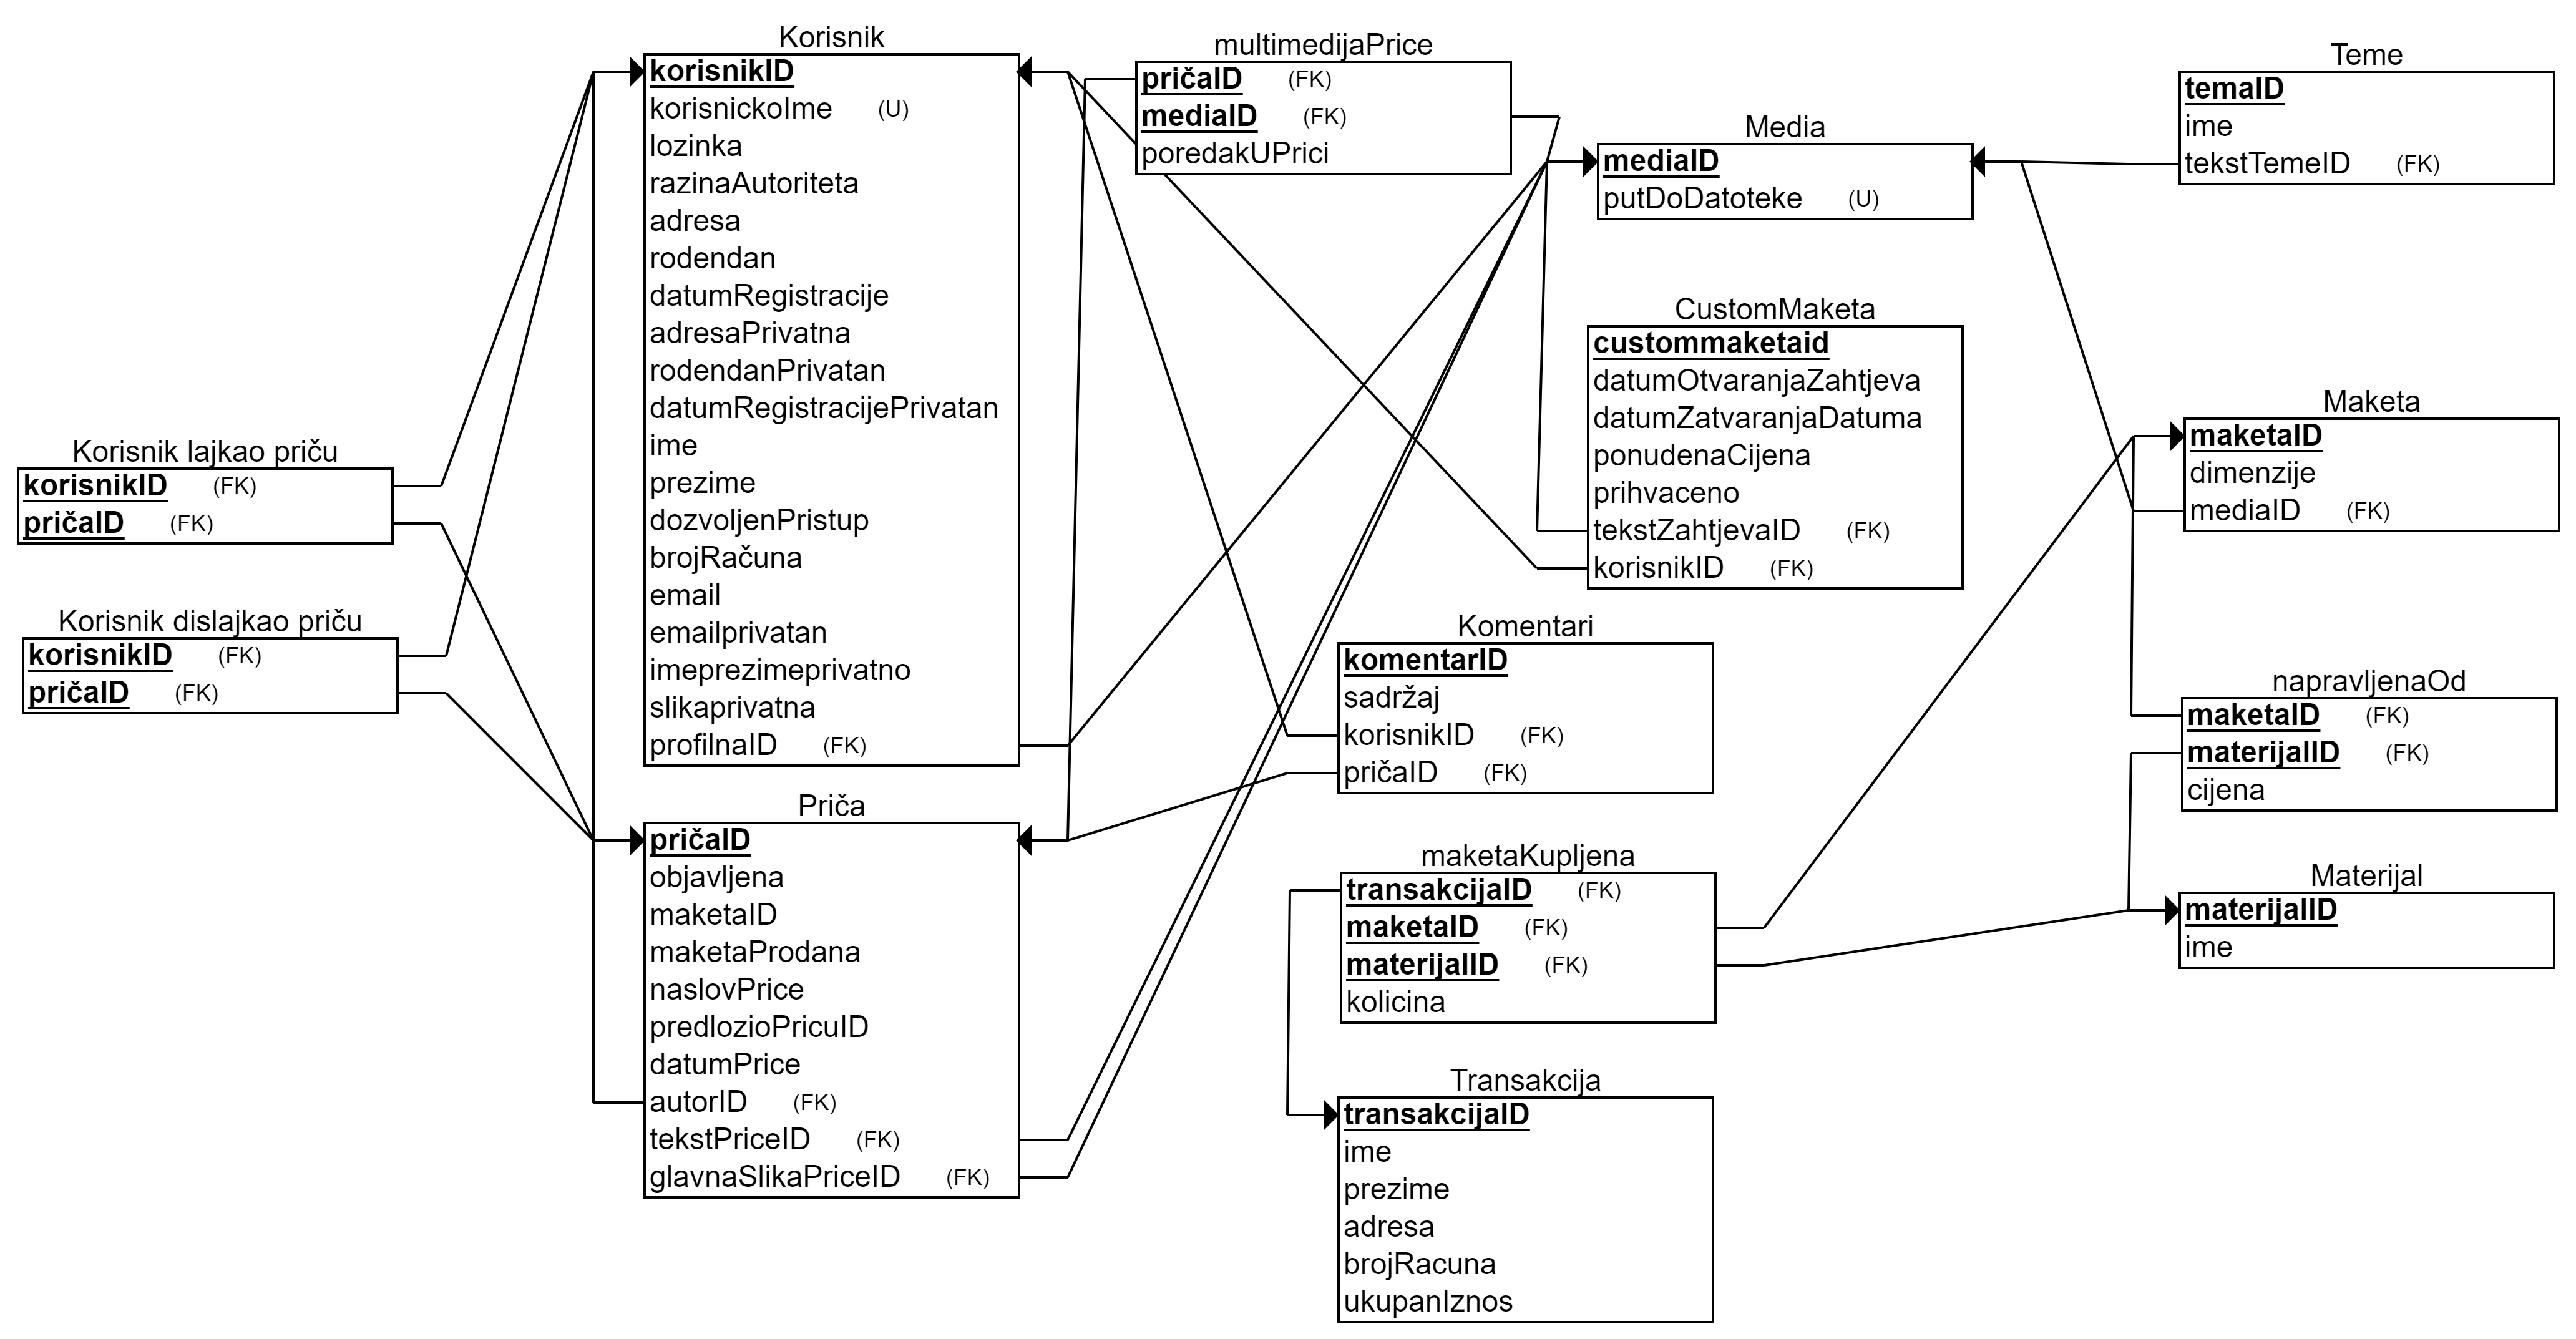
\includegraphics[width=1\linewidth]{slike/bazaRelShem}
			
			\eject
			
			
		\section{Dijagram razreda}
		
		Slike 4.2, 4.3 i 4.4 predstavljaju implementaciju razreda korištenih u backendu za prijenos podataka u korištenoj MTV arhitekturi. Slika 4.2 sadrži sve korištene razrede koji predstavljaju View tipove. Na slici 4.3 prikazane su Data Transfer Object tipovi podataka koji primaju podatake iz modela.  Slika 4.4 prikazuje razred modela onako kako su zapamćeni u bazi podataka te služe za direktnu interakciju s njom. WeTriedContext predstavlja sveukupan sadržaj korištene baze podataka.


		\begin{figure}[!h]
			\centering
			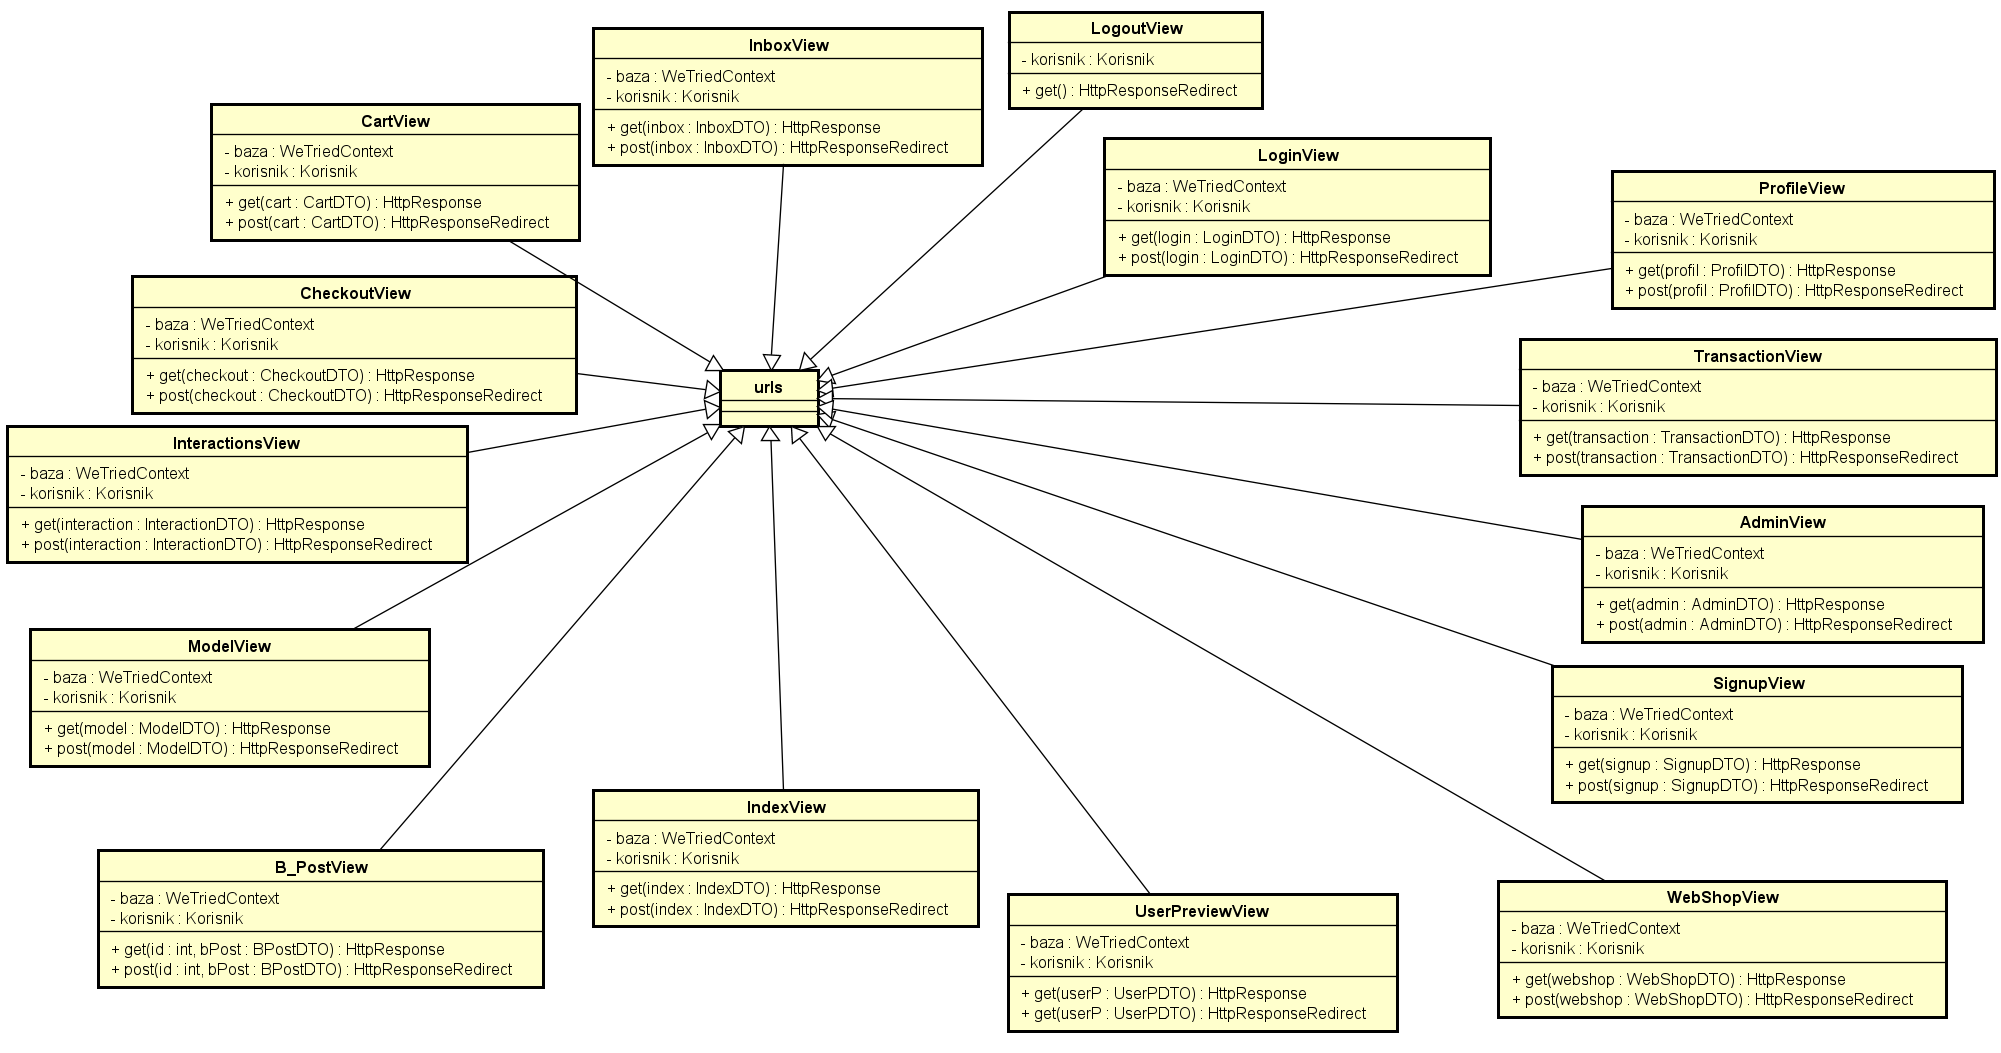
\includegraphics[width=1.1\linewidth, height=0.4\textheight]{slike/dijagram_razreda_1}
			\caption{Dijagram razreda - Views}
			\label{fig:dijagramrazreda1}
		\end{figure}
		
		
		
		
		\begin{figure}
			\centering
			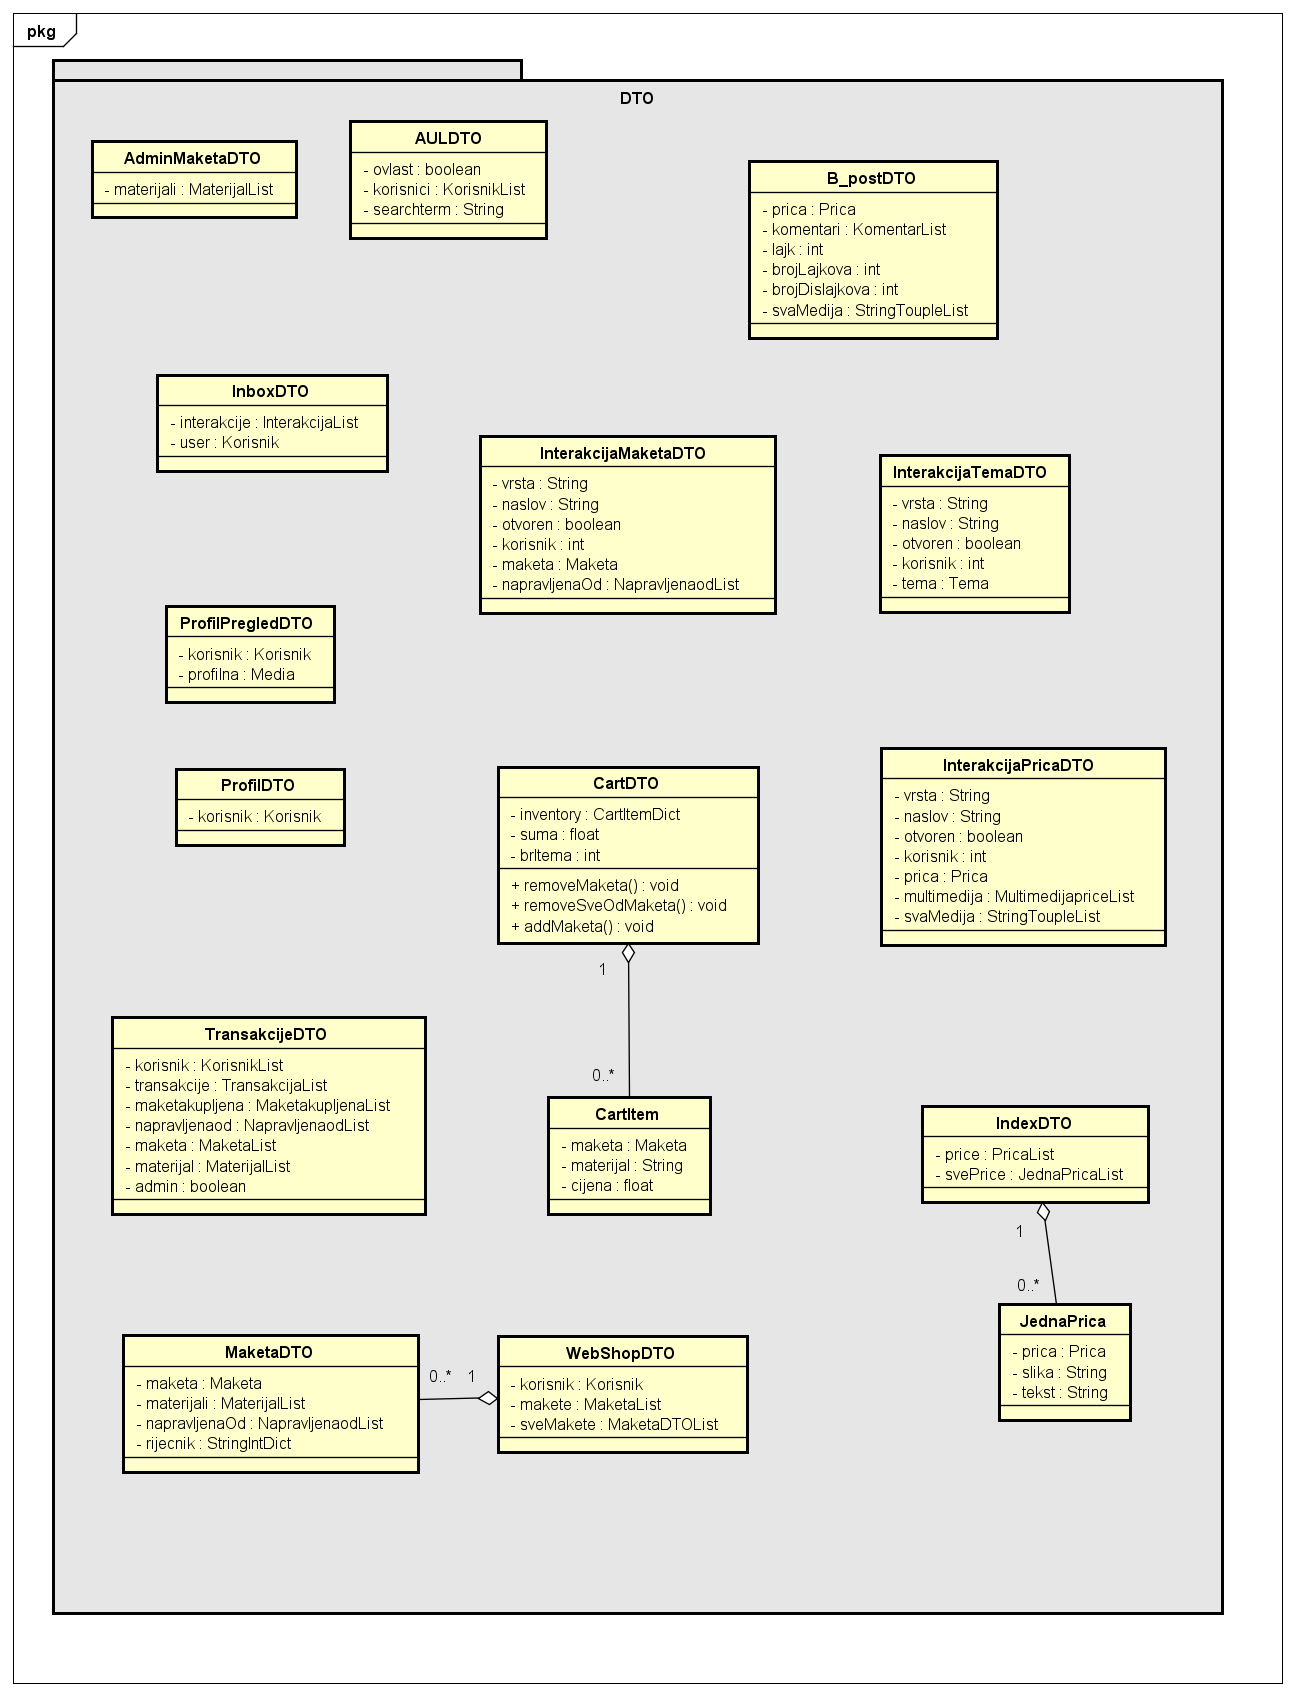
\includegraphics[width=1.0\linewidth]{slike/dijagram_razreda_2}
			\caption{Dijagram razreda - DTO}
			\label{fig:dijagramrazreda2}
		\end{figure}
		\begin{figure}
			\centering
			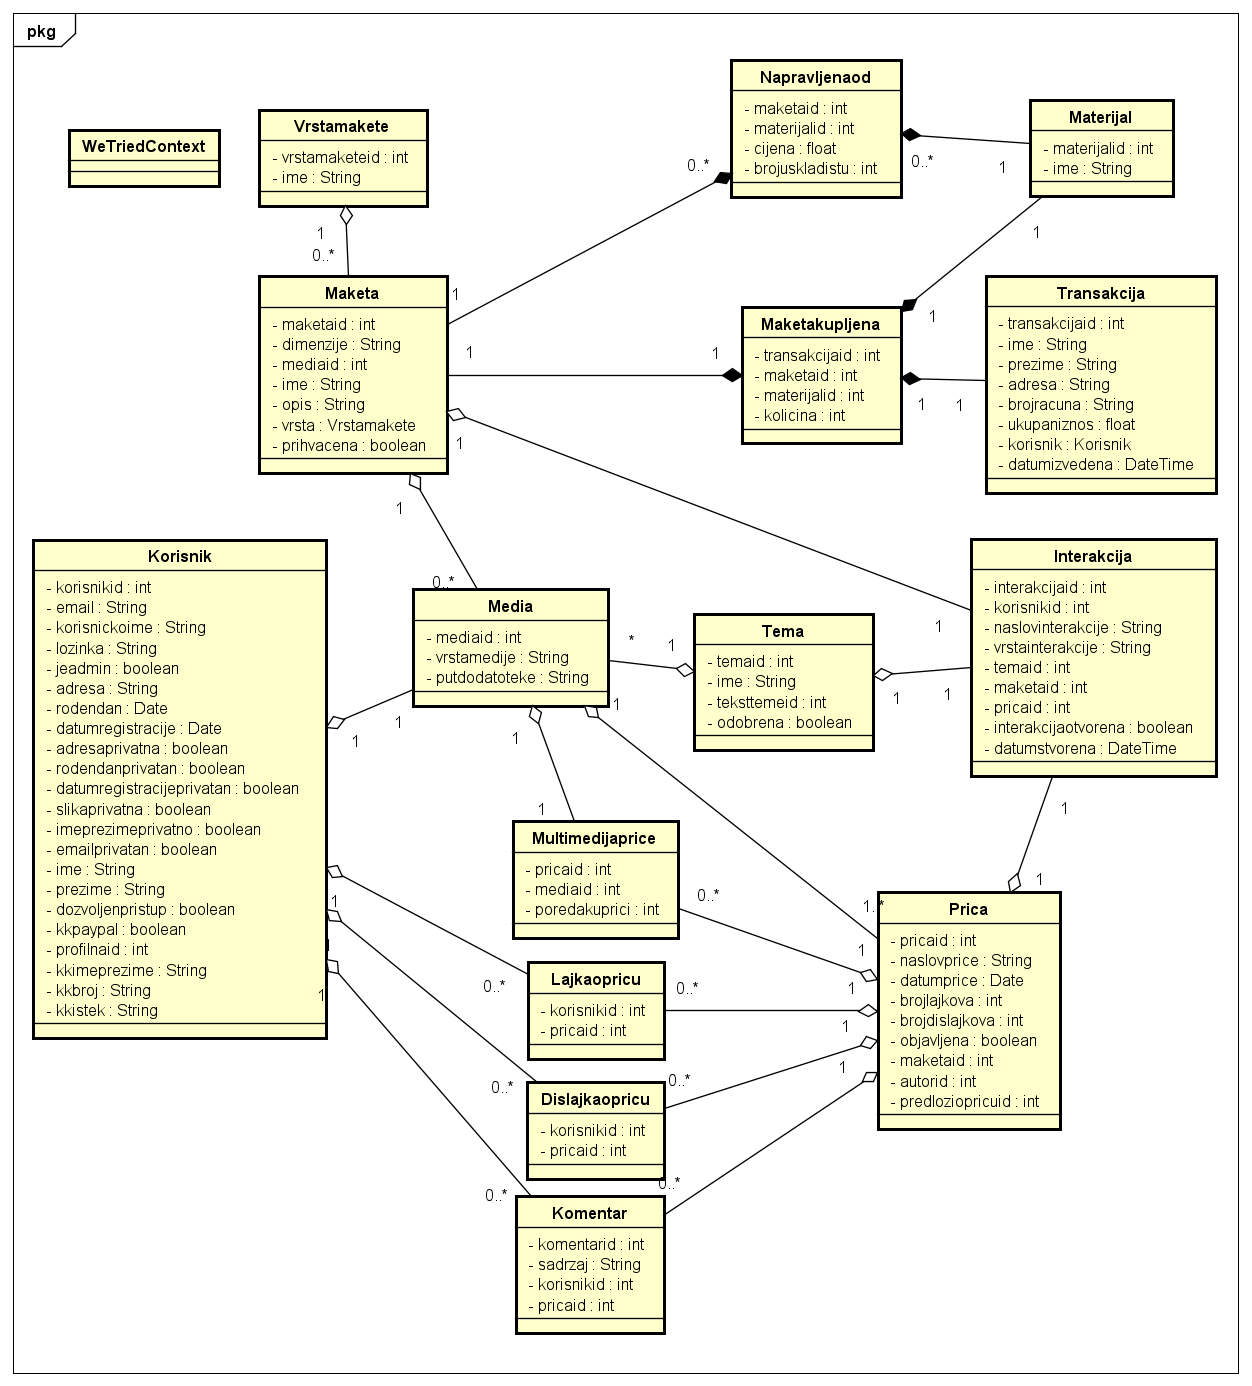
\includegraphics[width=1.0\linewidth]{slike/dijagram_razreda_3}
			\caption{Dijagram razreda - Models}
			\label{fig:dijagramrazreda3}
		\end{figure}
			\eject

	\section{Dijagram stanja}
	
		Prikazan je dijagram stanja za registriranog korisnika. Nakon prijave, klijentu se prikazuje početna stranica na kojoj može pregledati priče. Zaglavlje stranice je uvijek dostupno i kroz nju korisnik može uvijek otići na "Početnu stranicu", "Moj Profil", "Webshop", "Moje transakcije", "Košarica" i "Sandučić. Također, kroz zaglavlje stranice registrirani korisnik se uvijek može i odjaviti.
		
		
		\begin{figure}[!h]
			\centering
			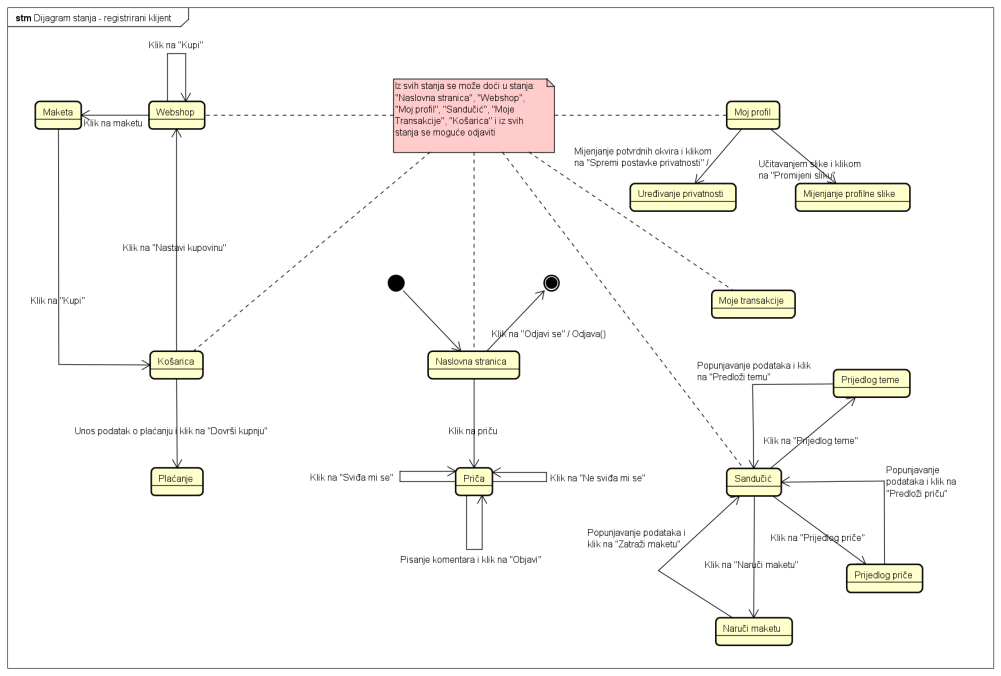
\includegraphics[width=1\linewidth]{slike/Dijagram_stanja_registrirani_klijent}
			\caption{Dijagram stanja - registrirani klijent}
			\label{fig:dijagramstanja}
		\end{figure}
		\eject
		
	\section{Dijagram aktivnosti}
		
		 Na dijagramu aktivnosti 4.5 prikazan je proces pregleda priče. Korisnik se prijavi u sustav te na početnoj stranici odabire priču makete koju želi detaljnije pregledati. U detaljnijem pregledu priče osim opisa makete korisniku se prikazuje broj lajkova i dislajkova za priču te komentari. Sam korisnik može odlučiti sviđa li mu se priča ili ne te ostaviti svoj komentar. Pregled priče prestaje odlaskom na neku drugu stranicu.
		
		
		\begin{figure}[!h]
			\centering
			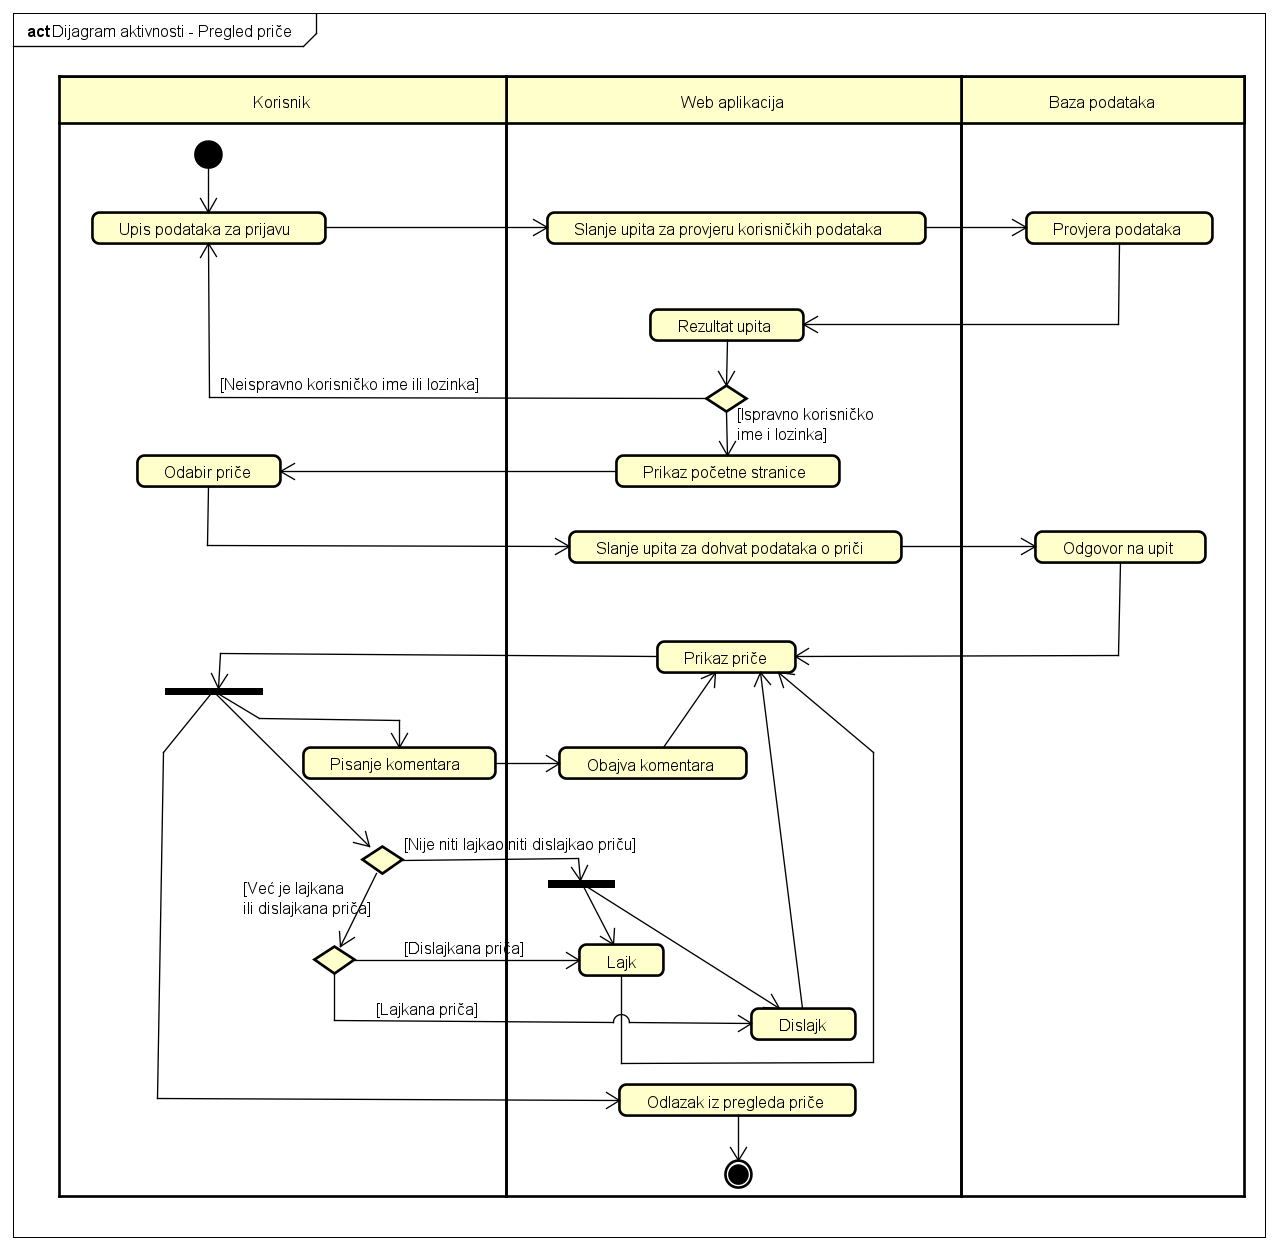
\includegraphics[width=1\linewidth]{slike/dijagram_aktivnosti}
			\caption{Dijagram aktivnosti - Pregled priče}
			\label{fig:dijagramaktivnosti}
		\end{figure}
	\eject
	\chapter{Implementacija i korisničko sučelje}
		
		
		\section{Korištene tehnologije i alati}
		
			 U svrhu ovog projekta korištene su sljedeće tehnologije i alati: Django i Bootstrap web programski okviri, sustav za upravljanje bazom podataka PostGreSQL, program pgAdmin, jezici HTML, CSS i JavaScript te biblioteku jQuery. \\
			 
			 
			 {Za pisanje backenda korišten je Django, web programski okvir utemeljen na jeziku Python. Preuzeti se može na ovoj  \href{https://www.djangoproject.com/}{\textbf{poveznici}}.
			 	
			 Baza podataka ostvarena je kroz sustav \href{https://www.postgresql.org/}{\textbf{PostGreSQL}} te uz pomoć programa \href{https://www.pgadmin.org/}{\textbf{pgAdmin}}.
			 
			 Frontend dio ostvaren je kroz korištenje standardnih jezika \href{https://www.w3schools.com/html/}{\textbf{HTML}},\href{https://www.w3schools.com/css/}{\textbf{CSS}} te \href{https://www.w3schools.com/js/DEFAULT.asp}{\textbf{JavaScript}}. Linkovi vode na stranice gdje se o njima može više saznati. 
			 
			 Uz navedene jezike korišteni su i programski okvir \href{https://getbootstrap.com/}{\textbf{Bootstrap}} pomoću kojeg su dobivene neke napredne funkcionalnosti frontenda te biblioteke \href{https://jquery.com/}{\textbf{jQuery}}.
			
			
			\eject 
		
	
		\section{Ispitivanje programskog rješenja}
			
			
			Ispitivanje se provodilo ručno. Kao temelj za ispitivanje koristili su se obrasci uporabe. Osim preciznog praćenja obrazaca također smo i nasumično navigirali po stranici u slučaju da negdje postoje greške u kodu (bugovi). Iako smo provjerili cijeli sustav radi pojednostavljenja u dokumentaciji prikazujemo samo 6 ispitnih slučajeva. Ispitali smo: UC2, UC3, UC10, UC18, UC20, UC24
			\\
			\\ 
			\textbf{Ispitni slučaj 1: Detaljan pregled priča}
			\\
			\textbf{Ulaz}
			\\
			\indent 1. Pritisak kursorom na određenu priču
			\\
			\textbf{Očekivani rezultat}
			\\
			\indent 1. Preusmjeravanje na stranicu odabrane priče
			\\
			\textbf{Rezultat}
			\\
			\indent Očekivani rezultat je zadovoljen te smo preusmjereni na stranicu za detaljan pregled priče koje smo odabrali. Slučaj je testiran i kao prijavljen korisnik i kao gost. Aplikacija je prošla test.
			\\ \\
			\begin{figure}[H]
				\centering
				\includegraphics[scale=0.34]{"slike/test1"}
				\caption{Rezultat ispitnog slučaja 1}
				\label{fig:rezultat-ispitnog-slucaja-1}
			\end{figure}
			
			\noindent \textbf{Ispitni slučaj 2: Komentiranje priče}
			\\
			\textbf{Ulaz}
			\\
			\indent 1. Navigacija do detaljnog pregleda priče \\
			\indent 2. Upisivanje samog komentara u predviđeno mjesto \\
			\indent 3. Pritisak gumba "Objavi"
			\\
			\textbf{Očekivani rezultat}
			\\
			\indent 1. Spremanje komentara u bazu za kasniji prikaz na stranici priče \\
			\indent 2. Osvježavanje stranice
			\\
			\textbf{Rezultat}
			\\
			\indent Očekivani rezultat je zadovoljen te se stranica osvježila te vidimo komentar koji smo ostavili. Komentar smo uspješno ostavili i kao gost i kao prijavljeni korisnik. Aplikacija je prošla test.
			\\ \\
			\begin{figure}[H]
				\centering
				\includegraphics[scale=0.34]{"slike/test2"}
				\caption{Rezultat ispitnog slučaja 2}
				\label{fig:rezultat-ispitnog-slucaja-2}
			\end{figure}
			
			\noindent \textbf{Ispitni slučaj 3: Predlaganje priče administratoru}
			\\
			\textbf{Ulaz}
			\\
			\indent 1. Navigacija stranice za prijedlog priče \\
			\indent 2. Odabir medije, naslova zahtjeva i naslova priče \\
			\indent 3. Pritisak gumba "Predloži priču"
			\\
			\textbf{Očekivani rezultat}
			\\
			\indent 1. Spremanje prijedloga priče u bazu \\
			\indent 2. Preusmjeravanje na stranicu sandučića
			\\
			\textbf{Rezultat}
			\\
			\indent Očekivani rezultat je zadovoljen. Preusmjereni smo na stranicu sandučića na kojoj vidimo još neobrađen zahtjev naše priče. Aplikacija je prošla test.
			\\ \\
			\begin{figure}[H]
				\centering
				\includegraphics[scale=0.34]{"slike/test3"}
				\caption{Rezultat ispitnog slučaja 3}
				\label{fig:rezultat-ispitnog-slucaja-3}
			\end{figure}
			
			\noindent \textbf{Ispitni slučaj 4: Pregled košarice}
			\\
			\textbf{Ulaz}
			\\
			\indent 1. Pritisak na gumb "Košarica" \\
			\textbf{Očekivani rezultat}
			\\
			\indent 1. Prikaz sadržaja u košarici, ukupne cijene te gumba za dovršavanje narudžbe. \\
			\textbf{Rezultat}
			\\
			\indent Očekivani rezultat je zadovoljen. Pritiskom na gumb košarica otvora se prikaz već navedenog sadržaja. Aplikacija je prošla test.
			\\ \\
			\begin{figure}[H]
				\centering
				\includegraphics[scale=0.34]{"slike/test4"}
				\caption{Rezultat ispitnog slučaja 4}
				\label{fig:rezultat-ispitnog-slucaja-4}
			\end{figure}
			
			\noindent \textbf{Ispitni slučaj 5: Promjena profilne slike}
			\\
			\textbf{Ulaz}
			\\
			\indent 1. Navigacija do stranice profila \\
			\indent 2. Odabir datoteke na računalu \\
			\indent 3. Pritisak gumba "Promijeni profilnu sliku" \\
			\textbf{Očekivani rezultat}
			\\
			\indent 1. Osvježavanje trenutne stranice na kojoj vidimo da je profilna slika promijenjena \\
			\textbf{Rezultat}
			\\
			\indent Očekivani rezultat nije zadovoljen. Namjerno nije odabrana nijedna slika, a gumb je svejedno pritisnut. Stranica se osvježila te profilna slika nije ažurirana.
			\\ \\
			\begin{figure}[H]
				\centering
				\includegraphics[scale=0.34]{"slike/test5"}
				\caption{Rezultat ispitnog slučaja 5}
				\label{fig:rezultat-ispitnog-slucaja-5}
			\end{figure}
			
			\noindent \textbf{Ispitni slučaj 6: Pregled registriranih korisnika}
			\\
			\textbf{Ulaz}
			\\
			\indent 1. Pritisak na ime korisnika bilo gdje na stranici \\
			\textbf{Očekivani rezultat}
			\\
			\indent 1. Prikaz profila odabranog korisnika. \\
			\textbf{Rezultat}
			\\
			\indent Očekivani rezultat je zadovoljen. Pritiskom na korisničko ime u komentarima preusmjereni smo na pregled profila odabranog korisnika. Aplikacija je prošla test.
			\\ \\
			\begin{figure}[H]
				\centering
				\includegraphics[scale=0.34]{"slike/test6"}
				\caption{Rezultat ispitnog slučaja 6}
				\label{fig:rezultat-ispitnog-slucaja-6}
			\end{figure}
			
			
		\subsection{Ispitivanje sustava}
			
			 
			 Korištenjem extenzije za Chrome preglednik Selenium isprobali smo sljedeće obrasce uporabe UC7, UC11, UC19 i UC4.
			 \\
			 \noindent \textbf{Ispitni slučaj 1: Pregled web shopa kao administrator}
			 \\
			 \textbf{Ulaz}
			 \\
			 \indent 1. Odabir gumba za prikaz webshopa iz padajućeg izbornika na zaglavlju stranice \\
			 \textbf{Očekivani rezultat}
			 \\
			 \indent 1. Prikaz webshopa. \\
			 \textbf{Rezultat}
			 \\
			 \indent Očekivani rezultat je zadovoljen. Pritiskom na spomenuti gumb preusmjereni smo na stranicu webshopa. Na slici je prikazano izvršavanje testa
			 \\ \\
			 \begin{figure}[H]
			 	\centering
			 	\includegraphics[scale=0.7]{"slike/test7"}
			 	\caption{Rezultat ispitnog slučaja 1}
			 	\label{fig:rezultat-ispitnog-slucaja-7}
			 \end{figure}
			 
			 \noindent \textbf{Ispitni slučaj 2: Ocjenjivanje priče}
			 \\
			 \textbf{Ulaz}
			 \\
			 \indent 1. Navigacija do stranice neke priče \\
			 \indent 2. Odabir opcije "sviđa mi se"/"ne sviđa mi se" \\
			 \textbf{Očekivani rezultat}
			 \\
			 \indent 1. Osvježenje stranice i ažuriranje broja ocjena priče\\
			 \textbf{Rezultat}
			 \\
			 \indent Očekivani rezultat je zadovoljen. Navigirali smo se do stranice priče i odabrali opciju "sviđa mi se" kao prijavljeni korisnik. Na slici je prikazano izvršavanje testa
			 \\ \\
			 \begin{figure}[H]
			 	\centering
			 	\includegraphics[scale=0.7]{"slike/test8"}
			 	\caption{Rezultat ispitnog slučaja 2}
			 	\label{fig:rezultat-ispitnog-slucaja-8}
			 \end{figure}
			 
			 \noindent \textbf{Ispitni slučaj 3: Upravljanje postavkama o privatnosti}
			 \\
			 \textbf{Ulaz}
			 \\
			 \indent 1. Navigacija do stranice vlastitog profila \\
			 \indent 2. Mijenjanje postavka privatnosti" \\
			 \indent 3. Pritisak gumba "Spremi postavke privatnosti" \\
			 \textbf{Očekivani rezultat}
			 \\
			 \indent 1. Osvježenje stranice i ažuriranje postavka privatnosti\\
			 \textbf{Rezultat}
			 \\
			 \indent Očekivani rezultat je zadovoljen. Navigirali smo se do stranice vlastitog profila i postavili adresu elektroničke pošte da bude privatna. Na slici je prikazano izvršavanje testa
			 \\ \\
			 \begin{figure}[H]
			 	\centering
			 	\includegraphics[scale=0.7]{"slike/test9"}
			 	\caption{Rezultat ispitnog slučaja 3}
			 	\label{fig:rezultat-ispitnog-slucaja-9}
			 \end{figure}
			 
			 \noindent \textbf{Ispitni slučaj 4: Registracija korisnika}
			 \\
			 \textbf{Ulaz}
			 \\
			 \indent 1. Navigacija do stranice za registraciju \\
			 \indent 2. Upisivanja podataka" \\
			 \indent 3. Pritisak gumba "Kreiraj račun" \\
			 \textbf{Očekivani rezultat}
			 \\
			 \indent 1. Registracija korisnika\\
			 \indent 2. Preusmjeravanje na početnu stranicu
			 \textbf{Rezultat}
			 \\
			 \indent Očekivani rezultat nije zadovoljen. Izostavili smo korisničko ime pri ispunjavanju podataka. Iskočila je poruka upozorenja da se to polje popuni. Na slici je prikazan krajnji dio izvršavanja testa.
			 \\ \\
			 \begin{figure}[H]
			 	\centering
			 	\includegraphics[scale=0.7]{"slike/test10"}
			 	\caption{Rezultat ispitnog slučaja 4}
			 	\label{fig:rezultat-ispitnog-slucaja-10}
			 \end{figure}
		
		
		\section{Dijagram razmještaja}
			
			Sustav je baziran na arhitekturi "klijent-poslužitelj". Koristimo HTTP za komunikaciju između korisnikovog uređaja i poslužitelja. Za posluživanje koristimo Heroku koji nudi platformu kao uslugu u oblaku. Heroku se sam brine o portovima, operativnim sustavima i okolinama poslužitelja pa nisu prikazani u dijagramu.
			
			\begin{figure}[!h]
				\centering
				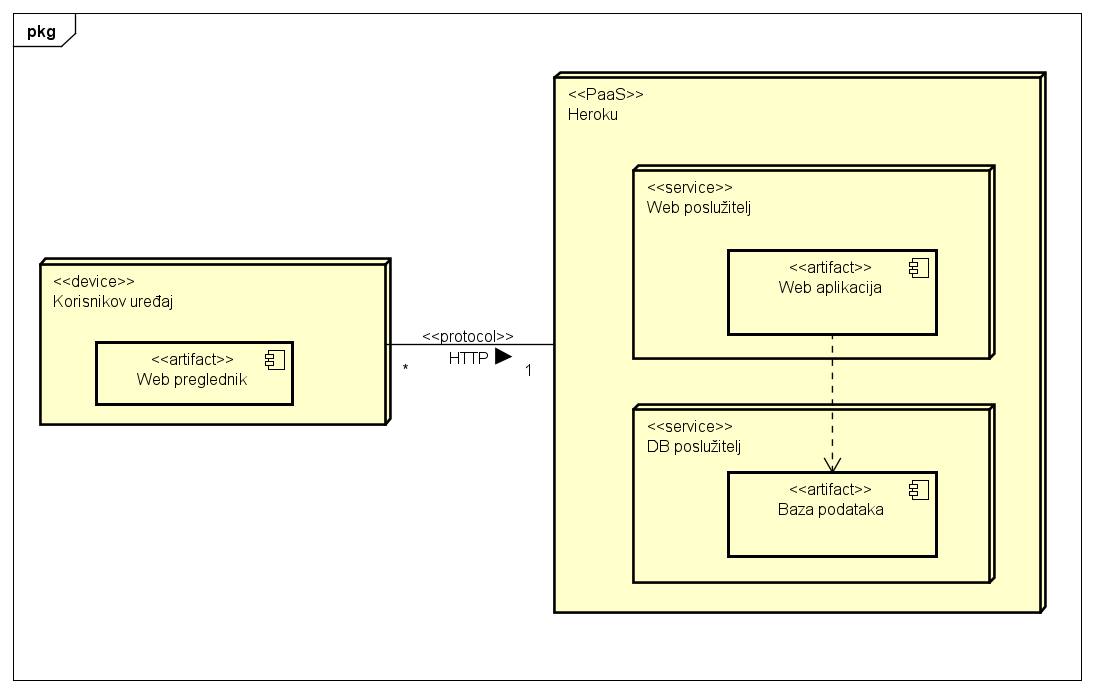
\includegraphics[width=1\linewidth]{slike/Dijagram_razmjestaja}
				\caption{Dijagram razmještaja}
				\label{fig:dijagramrazmjestaja}
			\end{figure}
			\eject
			
			\eject 
		
		\section{Upute za puštanje u pogon}
			\textbf{Instalacija Heroku poslužitelja}\\
			\\
			Potrebno je imati lokalno instalirani python verzije 3.8
			zajedno s najnovijom verzijom Django-a, najnoviju verziju Postgres-a, Git te besplatni Heroku račun.
			Potrebno je preuzeti Heroku Command Line Interface (CLI) koji je dostupan na https://cli-assets.heroku.com/heroku-x64.exe.
			Nakon toga potrebno je u Windows Command Prompt-u (cmd.exe) pokrenuti
			naredbu \verb|heroku login| koja će u zasebnom prozoru preglednika prikazati stranicu za login. \\
			\\
			\textbf{Konfiguracija aplikacije za Heroku}\\
			\\
			Kako bi se Heroku web aplikacija dobro konfigurirala potrebno je u
			Django server dodati 3 datoteke: \\
			1) requirements.txt s \\
			"Django==3.1.3 \\
			gunicorn==20.0.4 \\
			psycopg2-binary==2.8.6 \\
			pytz==2020.4 \\
			sqlparse==0.4.1 \\
			asgiref==3.3.0 \\
			dj-database-url==0.5.0 \\
			whitenoise==5.2.0 \\
			boto3==1.16.51 \\
			botocore==1.19.51 \\
			django-storages==1.11.1 \\
			jmespath==0.10.0 \\
			python-dateutil==2.8.1 \\
			s3transfer==0.3.3 \\
			six==1.15.0 \\
			urllib3==1.26.2" \\
			\\
			2) Procfile (bitno: Datoteka nema ekstenziju) s \\
			"web: gunicorn WeTried.wsgi --log-file -"
			\\
			3) runtime.txt s \\
			"python-3.8.6" \\
			\\
			\textbf{Stvaranje Heroku web aplikacije}\\
			\\
			Potrebno je imati lokalni git repozitorij koji se može stvoriti naredbom
			\verb|git init|.
			Pokretanjem naredbe 
			\verb|heroku create <name>| (naš name glasi "maketashop")
			stvara se heroku aplikacija i automatski se povezuje s lokalnim git repozitorijem.
			Nakon stvaranja aplikacije potrebno je dostaviti sam server pomoću naredbe \verb|git push heroku master|. Ako proces završi bez grešaka aplikacija je uspješno puštena u pogon, ostalo je samo povezati bazu s Djangom.
			\\
			\\
			\textbf{Konfiguriranje baze podataka}\\
			\\
			Heroku sam po sebi pri stvaranju python web aplikacije stvori addon
			postgresql tako da je potrebno samo u settings.py dodati \\
			\verb|"DATABASE_URL = <url>"| (url koji je generirao heroku) \\
			"DATABASES = {
				'default': dj\_database\_url.config(default=DATABASE\_URL)
			}"
			i \\
			"ALLOWED\_HOSTS = ['maketashop.herokuapp.com']". \\
			Nemojte zaboraviti maknuti konfiguraciju za korištenje lokalne baze podataka.\\
			\\
			\textbf{Upravljanje bazom podataka}\\
			\\
			Prije korištenja baze podataka potrebno je napraviti migracije te ih pokrenuti kako bi u bazi podataka bile sve tablice koje su potrebne za funkcioniranje baze podataka. To se radi tako što pokrenemo \verb|heroku run python manage.py makemigrations| koja napravi migracije, a zatim \verb|heroku run python manage.py migrate| koja te migracije primijeni.
			
			Budući da aplikacija velikim dijelom nema sadržaja dok korisnici ne počnu postavljati sadržaj, nije potrebno nikako populirati bazu podataka
			
			Da bismo vidjeli koji dodatak koristimo kako bismo se spojili na bazu podataka, pokrećemo naredbu \verb|heroku addons| koja nam daje sljedeći ispis:
			\begin{figure}[H]
				\centering
				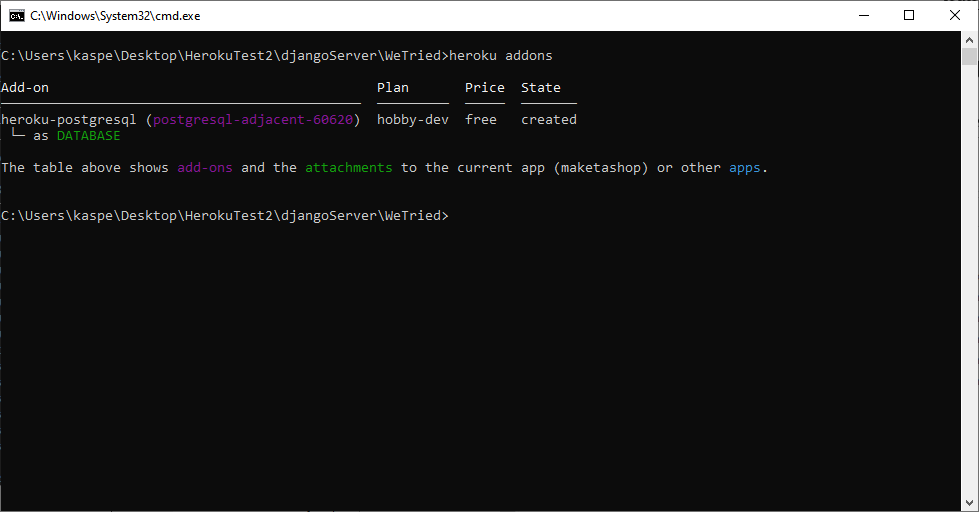
\includegraphics[width=1\linewidth]{slike/herokuPostgresql}
				\caption{Ispis naredbe heroku addons}
				\label{fig:herokuaddons}
			\end{figure}
			
			Ako želimo izravno upravljati bazom koristeći SQL upite kao vlasnik aplikacije, u naredbenom retku pokrećemo naredbu \verb|heroku pg:psql| koja nam otvara sučelje u kojemu možemo upisivati upite.
			
			\begin{figure}[H]
				\centering
				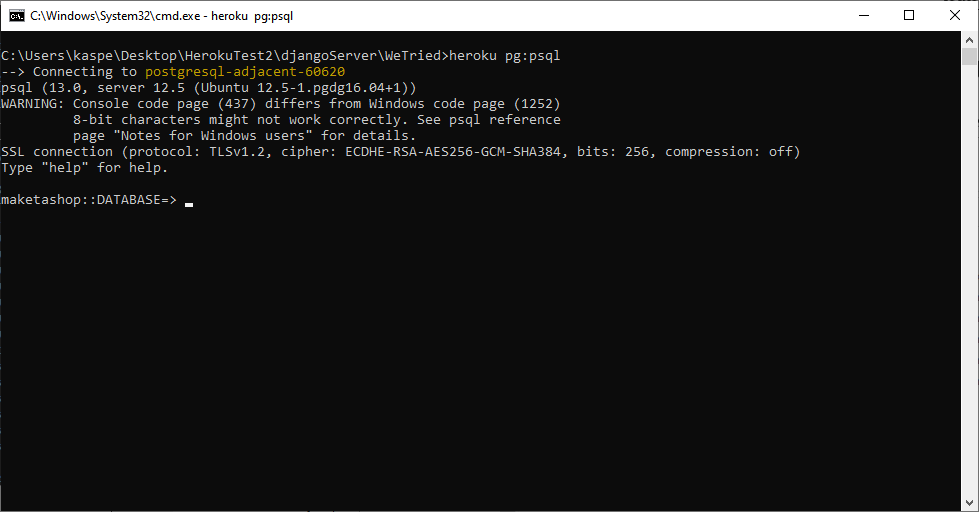
\includegraphics[width=1\linewidth]{slike/herokuPostgresql2}
				\caption{Ispis naredbe heroku pg:psql}
				\label{fig:pgpsql}
			\end{figure}
			Kada smo gotovi s postavljanjem upita, iz sučelja izlazimo naredbom \verb|\q|\\
			\\
			\textbf{Postavljanje posluživanja statičkih resursa}
			\\
			\\
			Budući da Django ne podržava posluživanje statičkih resursa u produkciji, potrebno je instalirati i konfigurirati paket whitenoise. Paket će biti instaliran budući da smo ga uključili u requirements.txt. Potrebno je još dodati sljedeće postavke u settings.py datoteku:\\
			\verb|BASE_DIR = os.path.dirname(os.path.dirname(os.path.abspath(__file__)))|\\
			\verb|STATIC_ROOT = os.path.join(BASE_DIR, 'staticfiles')|\\
			\verb|STATIC_URL = '/static/'|
			\begin{verbatim}
				STATICFILES_DIRS = (
					os.path.join(BASE_DIR, 'static'),
				)
			\end{verbatim}
			Osim toga, potrebno je dodati whitenoise middleware u MIDDLEWARE listu u datoteci settings.py. To seradi tako što samo dodamo string\\ \verb|'whitenoise.middleware.WhiteNoiseMiddleware',|\\ odmah nakon sigurnosnog middlewarea.
			\\
			\\
			\textbf{Postavljanje posluživanja korisničkih datoteka}
			\\
			\\
			Veliki dio funkcionalnosti aplikacije oslanja se na mogućnost korisnika da postavljaju svoje datoteke na server. Primjer toga je recimo sastavljanje priče ili kreiranje makete u web trgovini za koju je potrebno definirati sliku. Kako je heroku-ov datotečni sustav kratkotrajan (eng. \textit{ephemeral filesystem}), datoteke je potrebno spremiti na udaljeni poslužitelj i dohvaćati ga od tamo.\\
			Kako bismo ostvarili tu funkcionalnost odlučili smo koristiti Amazonov web servis S3. Da bi mogli spojiti se na AWS S3, potrebno je instalirati paket django-storages, zbog cega je on vec dodan u requirements.txt file, što znači da će biti instaliran prilikom puštanja aplikacije u pogon.\\
			Također, potrebno je registrirati se na amazonov servis. Na glavnoj stranici Amazon Web Services (\url{https://aws.amazon.com}), nalazi se gumb koji možemo kliknuti i unijeti podatke potrebne za registraciju. Nakon registracije. Kada pronađemo stranicu usluge S3, kreiramo 
			\eject 
	\chapter{Zaključak i budući rad}
		
		Zadatak dodijeljen našoj grupi bio je razvoj web aplikacije za objavljivanje multimedijskog sadržaja o maketama te mogućnost prodavanja maketa. Izrada samog projekta trajala je 15 tjedana kroz kojih je većinom prevladavao rad na implementaciji programskog rješenja, a dio vremena odvojili smo na pisanje dokumentacije projekta. Na samom početku projekta, izdvojili smo dio vremena za pisanje projektne dokumentacije koja je služila kao dobar predložak u procesu pisanja programske potpore. Projekt nam se ugrubo sastojao od dvije faze.
		
		\textbf	Prva faza većinom se sastojala od upoznavanja s novim pojmovima i tehnologijima. Nakon odabira željenih tehnologija, krenuli smo s implementacijom jednostavnijih funkcionalnosti naše web aplikacije kao što su jednostavnije korisničko sučelje, registracija i odjavljivanje korisnika, pregled vlastitog profila, početna stranica i online trgovina s pregledom priča o maketama. Početna stranica i online trgovina sadržavale su statičke podatke te su služile kao svojevrsan prototip za daljnji razvoj stranice. Uz dokumentaciju, veliki dio početne faze uključivalo je detaljno oblikovanje baze podataka.
		
		\textbf Druga faza započela je prebacivanjem backenda na objektno orijentiranu paradigmu. Nadalje, bilo je potrebno dinamički povezati sadržaje na stranicama. Osim nekoliko izmjena u bazi podataka započeli smo s implementacijom zahtjevnijih funkcionalnosti web aplikacije. Jedan od glavnih zadataka bio je napraviti sandučić koji služi za interakciju administratora i registriranog korisnika. Od zahtjevnijih zadataka ističe se implementacija procesa kupovine koji uključuje pregled i odabir maketa, prikazivanje željenih maketa u košarici te ispunjavanje traženog formulara koji predstavlja plaćanje putem interneta. Stekli smo znanje o postavljanju multimedijskog sadržaja na stranicu i daljnjem rukovanju tog sadržaja.
		
		\textbf Sudjelovanje na ovom projektu naučilo nas je komunikaciji između backenda i frontenda. Dobra podjela rada i organizacija bili su od velikog značaja za uspješno izvršavanje dodijeljenih zadatka. Glavna komunikacija vršila se putem platforme Discord. Moguća proširenja uključivala bi dodatne interaktivne funkcionalnosti korisnika i administratora. Tijekom projekta stekli smo bitna znanja o razvoju web aplikacija. Mislimo da uvijek postoji prostora za usavršavanje aplikacije no zadovoljni smo postignutim rezultatima.
		
		
		\eject 
	\chapter*{Popis literature}
		\addcontentsline{toc}{chapter}{Popis literature}
	 	
 		\textbf{\textit{Kontinuirano osvježavanje}}
	
		\textit{Popisati sve reference i literaturu koja je pomogla pri ostvarivanju projekta.}
		
		
		\begin{enumerate}
			
			
			\item  Programsko inženjerstvo, FER ZEMRIS, \url{http://www.fer.hr/predmet/proinz}
			
			\item  I. Sommerville, "Software engineering", 8th ed, Addison Wesley, 2007.
			
			\item  T.C.Lethbridge, R.Langaniere, "Object-Oriented Software Engineering", 2nd ed. McGraw-Hill, 2005.
			
			\item  I. Marsic, Software engineering book``, Department of Electrical and Computer Engineering, Rutgers University, \url{http://www.ece.rutgers.edu/~marsic/books/SE}
			
			\item  The Unified Modeling Language, \url{https://www.uml-diagrams.org/}
			
			\item  Astah Community, \url{http://astah.net/editions/uml-new}
		\end{enumerate}
		
		 
	
	
	\begingroup
	\renewcommand*\listfigurename{Indeks slika i dijagrama}
	%\renewcommand*\listtablename{Indeks tablica}
	%\let\clearpage\relax
	\listoffigures
	%\vspace{10mm}
	%\listoftables
	\endgroup
	\addcontentsline{toc}{chapter}{Indeks slika i dijagrama}


	
	\eject 
		
	\chapter*{Dodatak: Prikaz aktivnosti grupe}
		\addcontentsline{toc}{chapter}{Dodatak: Prikaz aktivnosti grupe}
		
		\section*{Dnevnik sastajanja}
		
		\begin{packed_enum}
			\item  sastanak
			
			\item[] \begin{packed_item}
				\item Datum: 5. listopada 2020.
				\item Prisustvovali: T.Hrestak, L.Novački, P.Pažur, L.Rabuzin, S.Sičić, I.Šarić, F.Zmiša
				\item Teme sastanka:
				\begin{packed_item}
					\item  uvodni sastanak s asistentom
					\item  opis i detaljnije objašnjenje projektnog zadatka
					\item  osnovne informacije o organizaciji projekta
					\item  razjašnjene temeljne dileme oko funkcionalnosti
				\end{packed_item}
			\end{packed_item}
		
			\item  sastanak
			
			\item[] \begin{packed_item}
				\item Datum: 14. listopada 2020.
				\item Prisustvovali: T.Hrestak, L.Novački, P.Pažur, L.Rabuzin, S.Sičić, I.Šarić, F.Zmiša
				\item Teme sastanka:
				\begin{packed_item}
					\item  pojašnjavanje rada s gitom i \LaTeX om
					\item  postavljena pravila o radu s dokumentacijom
					\item  uspostavljeni kanali komunikacije i organizacije (Discord i Trello)
					\item  podijeljen posao oko rada na poglavlju 2 i 3
				\end{packed_item}
			\end{packed_item}
		
			\item  sastanak
			
			\item[] \begin{packed_item}
				\item Datum: 17. listopada 2020.
				\item Prisustvovali: T.Hrestak, L.Novački, P.Pažur, L.Rabuzin, S.Sičić, I.Šarić, F.Zmiša
				\item Teme sastanka:
				\begin{packed_item}
					\item  zajednički rad na definiciji obrazaca uporabe
				\end{packed_item}
			\end{packed_item}
		
			\item  sastanak
			
			\item[] \begin{packed_item}
				\item Datum: 19. listopada 2020.
				\item Prisustvovali: T.Hrestak, L.Novački, P.Pažur, L.Rabuzin, S.Sičić, I.Šarić, F.Zmiša
				\item Teme sastanka:
				\begin{packed_item}
					\item  planiranje daljnih aktivnosti
					\item  delegacija posla:
					\begin{packed_item}
						\item  UML dijagrami za obrasce uporabe - Hrestak i Zmiša
						\item  prebacivanje opisa obrazaca uporabe iz google docs-a u službenu dokumentaciju: Sičić
						\item  sekvencijski dijagrami - Novački
						\item  privremeno sučelje - Rabuzin, Sičić i Šarić
						\item  baza podataka - Pažur
					\end{packed_item}
				\end{packed_item}
			\end{packed_item}
		
				\item  sastanak
			
			\item[] \begin{packed_item}
				\item Datum: 29. listopada 2020.
				\item Prisustvovali: T.Hrestak, L.Novački, P.Pažur, L.Rabuzin, S.Sičić, I.Šarić, F.Zmiša
				\item Teme sastanka:
				\begin{packed_item}
					\item Predstavljanje rezultata rada svake od grupa kroz posljednjih 10 dana
					\item Imenovanje voditelja backend tima i frontend tima:
						\begin{packed_item}
						\item  Backend: Hrestak i Zmiša
						\item  Frontend: Rabuzin
					\end{packed_item}
					\item Dogovoren rok do kada ćemo proučavati literaturu o korištenim tehnologijama - 31. listopada 2020.
				\end{packed_item}
			
			\end{packed_item}
		
		\item sastanak
		
		\item[] \begin{packed_item}
			\item Datum: 5. studenog 2020.
			\item Prisustvovali: T.Hrestak, L.Novački, L.Rabuzin, I.Šarić, F.Zmiša
			\item Teme sastanka:
			\begin{packed_item}
				\item Kratki pregled već obavljenog posla
				\item Kratki pregled rokova i plana za rad oko projekta
				\item Dogovor oko zajedničkog rada u subotu 7. studenog 2020.
			\end{packed_item}
			
		\end{packed_item}
	
	\item sastanak
	
	\item[] \begin{packed_item}
		\item Datum: 7. studenog 2020.
		\item Prisustvovali: T.Hrestak, L.Novački, L.Rabuzin, I.Šarić, F.Zmiša
		\item Teme sastanka:
		\begin{packed_item}
			\item Zajednički rad na implementaciji:
			\begin{packed_item}
				\item  View-ovi prebačeni iz skriptnog oblika u objektni
				\item  Forme prebačene u objektni oblik
				\item  Prosljeđivanje podataka o korisnicima i pričama iz baze na frontend
				\item  Uređivanje vizualnog izgleda
				\item  Povezivanje backenda i frontenda
			\end{packed_item}
		\end{packed_item}
		
	\end{packed_item}

	\item sastanak

	\item[] \begin{packed_item}
		\item Datum: 8. studenog 2020.
		\item Prisustvovali: T.Hrestak, L.Novački, P.Pažur, L.Rabuzin, S.Sičić, I.Šarić, F.Zmiša
		\item Teme sastanka:
		\begin{packed_item}
			\item Zajednički rad na implementaciji:
			\begin{packed_item}
				\item  Implementirana funkcionalnost ocjenjivanja priče
				\item  Implementirana funkcionalnost komentiranja
				\item  Uređen prikaz minijatura priča na glavnoj stranici
				\item  Dodane poveznice na upravljanje profilom ovisno je li korisnik prijavljen ili ne
			\end{packed_item}
		\end{packed_item}
	

		
	\end{packed_item}
	
		\item  sastanak
	
	\item[] \begin{packed_item}
		\item Datum: 3. prosinca 2020.
		\item Prisustvovali: T.Hrestak, L.Novački, P.Pažur, L.Rabuzin, S.Sičić, I.Šarić, F.Zmiša
		\item Teme sastanka:
		\begin{packed_item}
			\item  definiranje zadataka za rad na razvoju do kraja projekta
			\item  podjela posla na razvoju do kraja projekta
			\item  odlučivanje o restrukturiranju načina proslijeđivanja podataka s poslužitelja na klijent (uvođenje DTO-ova)
		\end{packed_item}
	\end{packed_item}
	
	\item  sastanak
	
	\item[] \begin{packed_item}
		\item Datum: 20. prosinca 2020.
		\item Prisustvovali: T.Hrestak, L.Novački, P.Pažur, L.Rabuzin, S.Sičić, I.Šarić, F.Zmiša
		\item Teme sastanka:
		\begin{packed_item}
			\item  cjelodnevni zajednički rad na projektu
		\end{packed_item}
	\end{packed_item}
	
	\item  sastanak
	
	\item[] \begin{packed_item}
		\item Datum: 28. prosinca 2020.
		\item Prisustvovali: T.Hrestak, L.Novački, P.Pažur, L.Rabuzin, S.Sičić, I.Šarić, F.Zmiša
		\item Teme sastanka:
		\begin{packed_item}
			\item  cjelodnevni zajednički rad na projektu
			\item  organizacija rada tijekom ostatka praznika
		\end{packed_item}
	\end{packed_item}
	
	\item  sastanak
	
	\item[] \begin{packed_item}
		\item Datum: 28. prosinca 2020.
		\item Prisustvovali: T.Hrestak, L.Novački, P.Pažur, L.Rabuzin, S.Sičić, I.Šarić, F.Zmiša
		\item Teme sastanka:
		\begin{packed_item}
			\item  cjelodnevni zajednički rad na projektu
			\item  organizacija rada tijekom ostatka praznika
		\end{packed_item}
	\end{packed_item}
	
	\item  sastanak
	
	\item[] \begin{packed_item}
		\item Datum: 4. siječnja 2021.
		\item Prisustvovali: T.Hrestak, L.Novački, P.Pažur, L.Rabuzin, S.Sičić, I.Šarić, F.Zmiša
		\item Teme sastanka:
		\begin{packed_item}
			\item  pregled implementiranih funkcionalnosti
			\item  delegiranje posla oko dokumentacije
			\item  dogovor oko vremenskog okvira završnih aktivnosti
		\end{packed_item}
	\end{packed_item}
	
	\item  sastanak
	
	\item[] \begin{packed_item}
		\item Datum: 11. siječnja 2021.
		\item Prisustvovali: Igor stančin, T.Hrestak, L.Novački, P.Pažur, L.Rabuzin, S.Sičić, I.Šarić, F.Zmiša
		\item Teme sastanka:
		\begin{packed_item}
			\item  Demonstracija alfa verzije aplikacije asistentu
		\end{packed_item}
	\end{packed_item}
	
	\item  sastanak
	
	\item[] \begin{packed_item}
		\item Datum: 12. siječnja 2021.
		\item Prisustvovali: L.Novački, L.Rabuzin, F.Zmiša
		\item Teme sastanka:
		\begin{packed_item}
			\item  Deployanje aplikacije
		\end{packed_item}
	\end{packed_item}			
			%
			
		\end{packed_enum}
		
		\eject
		\section*{Tablica aktivnosti}
		
			\begin{longtabu} to \textwidth {|X[7, l]|X[1, c]|X[1, c]|X[1, c]|X[1, c]|X[1, c]|X[1, c]|X[1, c]|}
								
				\cline{2-8} \multicolumn{1}{c|}{\textbf{}} &     \multicolumn{1}{c|}{\rotatebox{90}{\textbf{Lovro Rabuzin }}} & \multicolumn{1}{c|}{\rotatebox{90}{\textbf{Tvrtko Hrestak }}} &	\multicolumn{1}{c|}{\rotatebox{90}{\textbf{Leon Novački }}} &	\multicolumn{1}{c|}{\rotatebox{90}{\textbf{Patrik Pažur }}} &
				\multicolumn{1}{c|}{\rotatebox{90}{\textbf{Sara Sičić }}} &
				\multicolumn{1}{c|}{\rotatebox{90}{\textbf{Ivona Šarić }}} &	\multicolumn{1}{c|}{\rotatebox{90}{\textbf{Filip Zmiša }}} \\ \hline 
				\endfirsthead
				
			
				\cline{2-8} \multicolumn{1}{c|}{\textbf{}} &     \multicolumn{1}{c|}{\rotatebox{90}{\textbf{Ime Prezime voditelja}}} & \multicolumn{1}{c|}{\rotatebox{90}{\textbf{Ime Prezime }}} &	\multicolumn{1}{c|}{\rotatebox{90}{\textbf{Ime Prezime }}} &
				\multicolumn{1}{c|}{\rotatebox{90}{\textbf{Ime Prezime }}} &	\multicolumn{1}{c|}{\rotatebox{90}{\textbf{Ime Prezime }}} &
				\multicolumn{1}{c|}{\rotatebox{90}{\textbf{Ime Prezime }}} &	\multicolumn{1}{c|}{\rotatebox{90}{\textbf{Ime Prezime }}} \\ \hline 
				\endhead
				
				
				\endfoot
							
				 
				\endlastfoot
				
				Upravljanje projektom 		& 6 &  &  &  &  &  & \\ \hline
				Opis projektnog zadatka 	& 5 &  &  &  &  & 5.5 & \\ \hline
				
				Funkcionalni zahtjevi       & 1 &  &  &  & 2 &  &  \\ \hline
				Opis pojedinih obrazaca 	& 3.5 & 2.5 & 2 & 2 & 2 & 2.5 & 2.5 \\ \hline
				Dijagram obrazaca 			&  & 4.5 &  &  &  & & 4.5  \\ \hline
				Sekvencijski dijagrami 		&  &  & 3.5 &  &  &  &  \\ \hline
				Opis ostalih zahtjeva 		&  &  &  &  & 0.5 &  &  \\ \hline

				Arhitektura i dizajn sustava	 &  &  &  &  &  & 1 &  \\ \hline
				Baza podataka				&  &  &  & 3.5 &  &  &   \\ \hline
				Dijagram razreda 			&  & 6 &  &  &  &  &  6 \\ \hline
				Dijagram stanja				&  &  & 2 &  &  &  &  \\ \hline
				Dijagram aktivnosti 		&  &  &  &  &  & 2 &  \\ \hline
				Dijagram komponenti			&  &  &  &  & 2 &  &  \\ \hline
				Korištene tehnologije i alati 		&  &  &  & 1 &  &  &  \\ \hline
				Ispitivanje programskog rješenja 	&  &  &  & 4 &  &  &  \\ \hline
				Dijagram razmještaja			&  &  & 2 &  &  &  &  \\ \hline
				Upute za puštanje u pogon 		& 1 &  &  &  &  &  & 1 \\ \hline 
				Dnevnik sastajanja 			& 2 &  & 0.5 &  &  & 2 &  \\ \hline
				Zaključak i budući rad 		& & 1 &  &  &  & 1 &  \\  \hline
				Popis literature 			& 0.5 &  &  &  &  & 0.5 & 0.5 \\  \hline
				&  &  &  &  &  &  &  \\ \hline \hline
				Izrada baze podataka 		&  & 1 &  & 9 &  &  & 1 \\ \hline 
				Back end 			& 9 & 51 & 8 & 23 &  & 0.5 & 51 \\  \hline
				Front end			& 34 &  &  & 5 & 18 & 33 & 0.5 \\ \hline
				Deploy			& 9 &  &  &  &  &  & 3 \\ \hline
				Upravljanje atmosferom			&  &  &  &  &  & 2 &  \\ \hline
				
				
			\end{longtabu}
					
					
		\eject
		
		\section*{Dijagrami pregleda promjena}
		
		\textbf{\textit{dio 2. revizije}}\\
		
		\textit{Prenijeti dijagram pregleda promjena nad datotekama projekta. Potrebno je na kraju projekta generirane grafove s gitlaba prenijeti u ovo poglavlje dokumentacije. Dijagrami za vlastiti projekt se mogu preuzeti s gitlab.com stranice, u izborniku Repository, pritiskom na stavku Contributors.}
	


\end{document} %naredbe i tekst nakon ove naredbe ne ulaze u izgrađen dokument 


